%% =====================================================================
%%  An Experimental Analysis of MongoDB and PostgreSQL Performance
%%  Under Varying Data Volumes, Query Complexities, and Indexing Strategies
%%
%%  Formatted to match a standard two-column conference template:
%%    * A4, 1-inch margins, Times New Roman look (newtxtext/newtxmath)
%%    * Single-column title / author block / Abstract / Index terms
%%    * Two-column body from Section I onwards
%%    * Section headings: Roman numeral, bold, all-caps (I. INTRODUCTION)
%%    * Figure captions below figures ("Figure N: ..."),
%%      table captions above tables
%%    * Numbered equations, running page header, centred page numbers
%%    * Closing star ornament
%%
%%  Compile with:  pdflatex main.tex   (or xelatex / lualatex)
%% =====================================================================

\documentclass[10pt,a4paper,twocolumn]{article}

% ── Encoding & fonts (Times New Roman appearance) ────────────────────
\usepackage[T1]{fontenc}
\usepackage[utf8]{inputenc}
\usepackage{amsmath}
\usepackage{newtxtext,newtxmath}
\usepackage{textcomp}

% ── Page geometry ─────────────────────────────────────────────────────
\usepackage[a4paper,
            left=1in, right=1in, top=1in, bottom=1in,
            headheight=12pt, headsep=4pt, footskip=30pt,
            columnsep=15.5pt]{geometry}

% ── General packages ──────────────────────────────────────────────────
\usepackage{graphicx}
\usepackage{xcolor}
\usepackage{booktabs}
\usepackage{array}
\usepackage{adjustbox}
\usepackage{cite}
\usepackage{enumitem}
\usepackage{dblfloatfix}
\usepackage{caption}
\usepackage{titlesec}
\usepackage{fancyhdr}
\usepackage[hidelinks]{hyperref}

\graphicspath{{./}{./figures/}}

% ── Convenience macros ────────────────────────────────────────────────
\newcommand{\PaperTitle}{An Experimental Analysis of MongoDB and PostgreSQL
  Performance Under Varying Data Volumes, Query Complexities, and Indexing Strategies}
\newcommand{\RunningHeader}{AN EXPERIMENTAL ANALYSIS OF MONGODB AND POSTGRESQL PERFORMANCE}

% ── Paragraph settings ────────────────────────────────────────────────
\setlength{\parindent}{0.3in}
\setlength{\parskip}{0.7pt plus 0.3pt}
\setlist{nosep, leftmargin=1.4em, labelsep=0.5em}

% ── Header / footer ───────────────────────────────────────────────────
\fancypagestyle{main}{%
  \fancyhf{}%
  \fancyhead[C]{\footnotesize\bfseries\RunningHeader}%
  \fancyfoot[C]{\footnotesize\thepage}%
  \renewcommand{\headrulewidth}{0.5pt}%
  \renewcommand{\footrulewidth}{0.5pt}%
}
\fancypagestyle{plain}{%
  \fancyhf{}%
  \fancyfoot[C]{\footnotesize\thepage}%
  \renewcommand{\headrulewidth}{0pt}%
  \renewcommand{\footrulewidth}{0.5pt}%
}
\pagestyle{main}

% ── Section headings ──────────────────────────────────────────────────
\renewcommand{\thesection}{\Roman{section}}
\renewcommand{\thesubsection}{\Alph{subsection}}
\renewcommand{\thesubsubsection}{\arabic{subsubsection}}

\titleformat{\section}[hang]
  {\normalfont\normalsize\bfseries}{\makebox[0.4in][l]{\thesection.}}{0pt}{\MakeUppercase}
\titlespacing*{\section}{0pt}{9pt plus 2pt minus 1pt}{4pt plus 1pt}

\titleformat{\subsection}[hang]
  {\normalfont\normalsize\bfseries\itshape}{\thesubsection.}{0.5em}{}
\titlespacing*{\subsection}{0pt}{6pt plus 1pt minus 1pt}{2pt}

\titleformat{\subsubsection}[runin]
  {\normalfont\normalsize\itshape}{\thesubsubsection)}{0.5em}{}[:]
\titlespacing*{\subsubsection}{\parindent}{4pt plus 1pt}{0.5em}

% ── Captions ──────────────────────────────────────────────────────────
\captionsetup{font=footnotesize, labelsep=colon, justification=justified,
              singlelinecheck=true, skip=4pt}
\captionsetup[figure]{labelfont=bf, textfont=bf, name=Figure}
\captionsetup[table]{labelfont=bf, labelsep=newline, justification=centering,
                     position=above, name=Table, skip=3pt}

% ── Float behaviour ───────────────────────────────────────────────────
\renewcommand{\topfraction}{0.9}
\renewcommand{\bottomfraction}{0.7}
\renewcommand{\textfraction}{0.07}
\renewcommand{\floatpagefraction}{0.75}
\renewcommand{\dbltopfraction}{0.9}
\renewcommand{\dblfloatpagefraction}{0.75}
\setcounter{topnumber}{3}
\setcounter{bottomnumber}{2}
\setcounter{totalnumber}{5}
\setcounter{dbltopnumber}{3}
\extrafloats{60}
% Compact float separation; retain 10 pt text and one-inch margins.
\setlength{\textfloatsep}{10pt plus 2pt minus 2pt}
\setlength{\floatsep}{8pt plus 2pt minus 2pt}
\setlength{\intextsep}{8pt plus 2pt minus 2pt}
\setlength{\dbltextfloatsep}{10pt plus 2pt minus 2pt}
\setlength{\dblfloatsep}{8pt plus 2pt minus 2pt}

% Verify the requested ten-page ceiling after all floats have been shipped.
\AtEndDocument{%
  \clearpage
  \ifnum\value{page}>11\relax
    \PackageError{manuscript}{Page limit exceeded: \number\numexpr\value{page}-1\relax\space pages}{The manuscript must occupy at most ten pages.}%
  \fi
}

% ── Reference list typography ─────────────────────────────────────────
\let\OldTheBibliography\thebibliography
\renewcommand{\thebibliography}[1]{%
  \OldTheBibliography{#1}\footnotesize
  \setlength{\itemsep}{2pt plus 0.5pt}\setlength{\parskip}{0pt}}

% =====================================================================
\begin{document}
% =====================================================================

% ── Title / author / abstract block (single column) ──────────────────
\twocolumn[%
\begin{center}
  {\fontsize{14}{17}\selectfont\bfseries\MakeUppercase{\PaperTitle}\par}
  \vspace{12pt}
  {\small\bfseries
    Dharaneesh S~L\textsuperscript{1}\qquad
    Dr.~Saranya K~G\textsuperscript{2}\par}
  \vspace{10pt}
  {\small
    \textsuperscript{1}Student,
    Department of Computer Science and Engineering,
    PSG College of Technology, Coimbatore, Tamil Nadu, India\par
    \textsuperscript{2}Associate Professor,
    Department of Computer Science and Engineering,
    PSG College of Technology, Coimbatore, Tamil Nadu, India\par}
  \vspace{8pt}
  {\small
    \textsuperscript{1}dharaneesh19112006@gmail.com\quad
    \textsuperscript{2}kgs.cse@psgtech.ac.in\par}
\end{center}
\vspace{4pt}
\noindent\rule{\textwidth}{0.5pt}
\vspace{4pt}

\noindent\textbf{Abstract:}
\textbf{Problem:} Selecting a relational or document database requires measurements that distinguish schema choices from deployment and execution costs. \textbf{Objective:} This study evaluates PostgreSQL and MongoDB across the planned scale factors 0.1, 0.5, and 1.0, three core query workloads, and two secondary-index configurations. \textbf{MongoDB vs.\ PostgreSQL:} Both systems use the same eight-entity, TPC-H-derived logical schema. \textbf{Experimental Methodology:} Each completed configuration uses three warm-up runs and ten measured runs. Client-side latency is recorded through full result retrieval, executed plans are retained, and output-matched comparisons use a two-sided Mann--Whitney $U$ test with Holm adjustment. A 60-second server-side query limit applies. \textbf{Main Performance Metrics:} The evidence records latency, batch CRUD throughput, allocated data and index storage, and execution-plan counters. Local server-process CPU and aggregate RSS were sampled with the stated accounting limitations. \textbf{Key Findings:} PostgreSQL had the lower observed median in 10 of the 10 complete core-query comparisons, and MongoDB in 0. Completed-comparison speedups ranged from $1.83\times$ to $232.46\times$. \textbf{Conclusion:} Both database servers ran on the same Windows host over loopback connections. The results characterize the recorded single-node settings, derived datasets, and warm-cache workloads. Workload-specific medians and indexing effects provide the basis for the reported comparisons. Incomplete or timed-out conditions are identified explicitly.

\vspace{6pt}
\noindent\textbf{\textit{Index terms:}} MongoDB, PostgreSQL, NoSQL, relational database,
TPC-H, benchmarking, indexing, query performance, execution plans, empirical evaluation.

\vspace{4pt}
\noindent\rule{\textwidth}{0.5pt}
\vspace{10pt}
]% end \twocolumn[...]

\thispagestyle{plain}

% =====================================================================
\section{Introduction}
% =====================================================================

\subsection{Background}
The volume of data that applications must store and query has influenced the design of database systems~\cite{stonebraker2005c}. A single platform may need to ingest both structured transaction records and semi-structured event logs at high rates. The choice of storage engine depends on how well it can ingest and index those records and serve the queries the application actually issues~\cite{pavlo2016relational}.

\subsection{Relational Databases}
Relational database management systems represent data in tables~\cite{codd1970relational}. PostgreSQL supports normalized schemas, SQL queries, foreign-key constraints, and ACID transactions. Its cost-based optimizer uses table statistics and assumptions about available memory to choose among physical operators, including sequential scans, index scans, and hash joins~\cite{postgresql_docs,postgresql_explain}.

\subsection{NoSQL and MongoDB}
MongoDB stores self-describing BSON documents in collections with flexible schemas~\cite{mongodb_docs}. Each document can contain a hierarchy of nested values. Sharding distributes data horizontally across machines. For the join workloads examined here, MongoDB expresses the query as a sequence of aggregation stages, including \texttt{\$lookup} for access to a related collection. PostgreSQL expresses the corresponding join through its cost-based relational planner~\cite{mongodb_aggregation,mongodb_explain}.

\subsection{Problem Statement}
Despite widespread use of both systems, published comparisons give limited guidance on when MongoDB will outperform a relational database or when the reverse will hold. If a benchmark embeds related records in MongoDB and places them in separate relational tables, the measured difference reflects both the engine and the decision to denormalize.

\subsection{Research Motivation}
To isolate the contribution of the engine, we held the logical schema constant. Varying data volume, query complexity, and indexing together allowed us to identify the workload conditions under which the performance advantage shifted between systems.

\subsection{Research Objective}
Our objective was to build a reproducible benchmark for measuring latency, throughput, and resource use in MongoDB and PostgreSQL under the same logical conditions, using equivalent datasets derived from TPC-H.

\subsection{Research Questions}
\begin{itemize}
  \item \textbf{RQ1:} How does data volume affect create, read, update, and delete (CRUD) performance in MongoDB and PostgreSQL?
  \item \textbf{RQ2:} How does query complexity affect response time in each system?
  \item \textbf{RQ3:} How do secondary indexes affect read and write performance?
  \item \textbf{RQ4:} How do the two systems compare in storage, CPU, and memory requirements?
  \item \textbf{RQ5:} Which workload characteristics favor MongoDB, and which favor PostgreSQL?
\end{itemize}

% =====================================================================
\section{Literature Review}
% =====================================================================

\textbf{Previous Research:}
Comparisons of relational and NoSQL systems have become more common over the past decade. Cattell~\cite{cattell2011scalable} surveyed scalable data stores, and Stonebraker and colleagues~\cite{stonebraker2007end} argued that different workloads call for different database architectures. Sadalage and Fowler~\cite{sadalage2012nosql} helped popularize polyglot persistence, the practice of using different stores for different parts of an application. Leavitt~\cite{leavitt2010nosql} and Mohamed \emph{et al.}~\cite{mohamed2014relational} examined the trade-offs involved in adopting NoSQL. Han \emph{et al.}~\cite{han2011survey} and Gessert \emph{et al.}~\cite{gessert2017nosql} classified systems by data model and consistency properties.

Empirical studies have compared MongoDB with MySQL, SQL Server, and PostgreSQL, respectively, in work by Gy\H{o}r\"{o}di \emph{et al.}~\cite{gyorodi2015comparative}, Parker \emph{et al.}~\cite{parker2013comparing}, and Jung \emph{et al.}~\cite{jung2015mongodb}. Boicea \emph{et al.}~\cite{boicea2012mongodb} compared MongoDB with Oracle. Li and Manoharan~\cite{li2013performance} examined mixed SQL and NoSQL workloads, while Abramova and Bernardino~\cite{abramova2013nosql} studied MongoDB and Cassandra. YCSB~\cite{cooper2010ycsb} and OLTP-Bench~\cite{difallah2013oltpbench} provide frameworks for benchmarking. Raasveldt \emph{et al.}~\cite{raasveldt2018fair} discuss the experimental controls needed for fair comparisons.

\subsection{Research Gap}
Earlier comparisons typically vary data volume for a simple CRUD workload or vary query complexity at a fixed volume. Fewer studies relate client-side latency to specific plan measurements, such as buffer hits and documents examined, while also testing the differences between engines with a nonparametric method.

\subsection{Hypotheses}
\begin{itemize}
  \item \textbf{H1:} Increasing dataset size increases execution time for both
        databases~\cite{gyorodi2015comparative,truica2015performance}.
  \item \textbf{H2:} Increasing query complexity increases response
        time~\cite{chaudhuri1998overview}.
  \item \textbf{H3:} Appropriate indexing substantially reduces query response
        time~\cite{graefe2011modern}.
  \item \textbf{H4:} Indexing introduces additional storage and write-maintenance overhead.
  \item \textbf{H5:} MongoDB and PostgreSQL exhibit meaningfully different performance
        profiles across workload types~\cite{stonebraker2005c}.
  \item \textbf{H6 (Expectation):} We expect PostgreSQL to perform better on analytical workloads that require multi-way joins and MongoDB to perform better on simple queries that access a single document~\cite{gessert2017nosql}.
\end{itemize}

% =====================================================================
\section{Dataset and Experimental Environment}
% =====================================================================

\subsection{TPC-H Dataset}
The datasets follow the repository\textquotesingle s TPC-H-derived generator~\cite{tpch_spec,poess2000tpch} at the planned scale factors $\mathrm{SF}\in\{0.1,0.5,1.0\}$. SF~0.1 was exported from the existing Atlas data. Larger datasets were generated with the repository\textquotesingle s deterministic seeds. These are derived data distributions and locally defined query identifiers. Each dataset contains all eight entities: \texttt{CUSTOMER}, \texttt{ORDERS}, \texttt{LINEITEM}, \texttt{PART}, \texttt{SUPPLIER}, \texttt{PARTSUPP}, \texttt{NATION}, and \texttt{REGION}.

\subsection{Hardware Configuration}
Table~\ref{tab:env} lists the verified client and PostgreSQL host environment and the database versions returned by the live servers. Both servers and the client run on this host. The initial Atlas dataset was exported before the local comparison.

\begin{table}[htbp]
\caption{Experimental Environment (Hardware and Software)}
\label{tab:env}
\centering
\renewcommand{\arraystretch}{1.25}
\begin{tabular}{@{}ll@{}}
\toprule
\textbf{Component}      & \textbf{Value} \\ \midrule
CPU                     & Intel Core i7-14650HX \\
RAM                     & 23.64\,GiB \\
Storage                 & Samsung 1\,TB SSD \\
Operating System        & Windows~11 \\
MongoDB Version         & 8.0.37 (local) \\
PostgreSQL Version      & 18.7 (local) \\
Python Version          & 3.14.7 \\
PyMongo driver          & 4.19.0 \\
Psycopg2 driver         & 2.9.13 \\
\bottomrule
\end{tabular}
\end{table}

\subsection{Software Stack}
The Python client uses PyMongo 4.19.0 and Psycopg2 2.9.13. Local MongoDB 8.0.37 uses WiredTiger and PostgreSQL reports version 18.7. PostgreSQL uses synchronous commit. MongoDB writes use acknowledged, journaled writes ($w=1$, journal=true). PostgreSQL uses shared\_buffers=128\,MiB, work\_mem=4\,MiB, and up to two parallel workers per gather. WiredTiger\textquotesingle s configured maximum cache is 1{,}073{,}741{,}824 bytes (1\,GiB). The configured settings therefore imply different cache budgets. Analysis uses pandas 3.0.6, NumPy 2.5.3, and SciPy 1.18.1.

% =====================================================================
\section{Proposed Framework}
% =====================================================================

\subsection{Architecture}
Figure~\ref{fig:arch} traces a benchmark run through five layers. The TPC-H data generator writes CSV files for each scale factor, and the data loader imports them into the two databases. The Python benchmark engine runs the queries, switches the index configuration, and records the measurements. The statistical analysis layer reads the resulting CSV files and applies the Mann--Whitney $U$ test.

\begin{figure}[htbp]
  \centering
  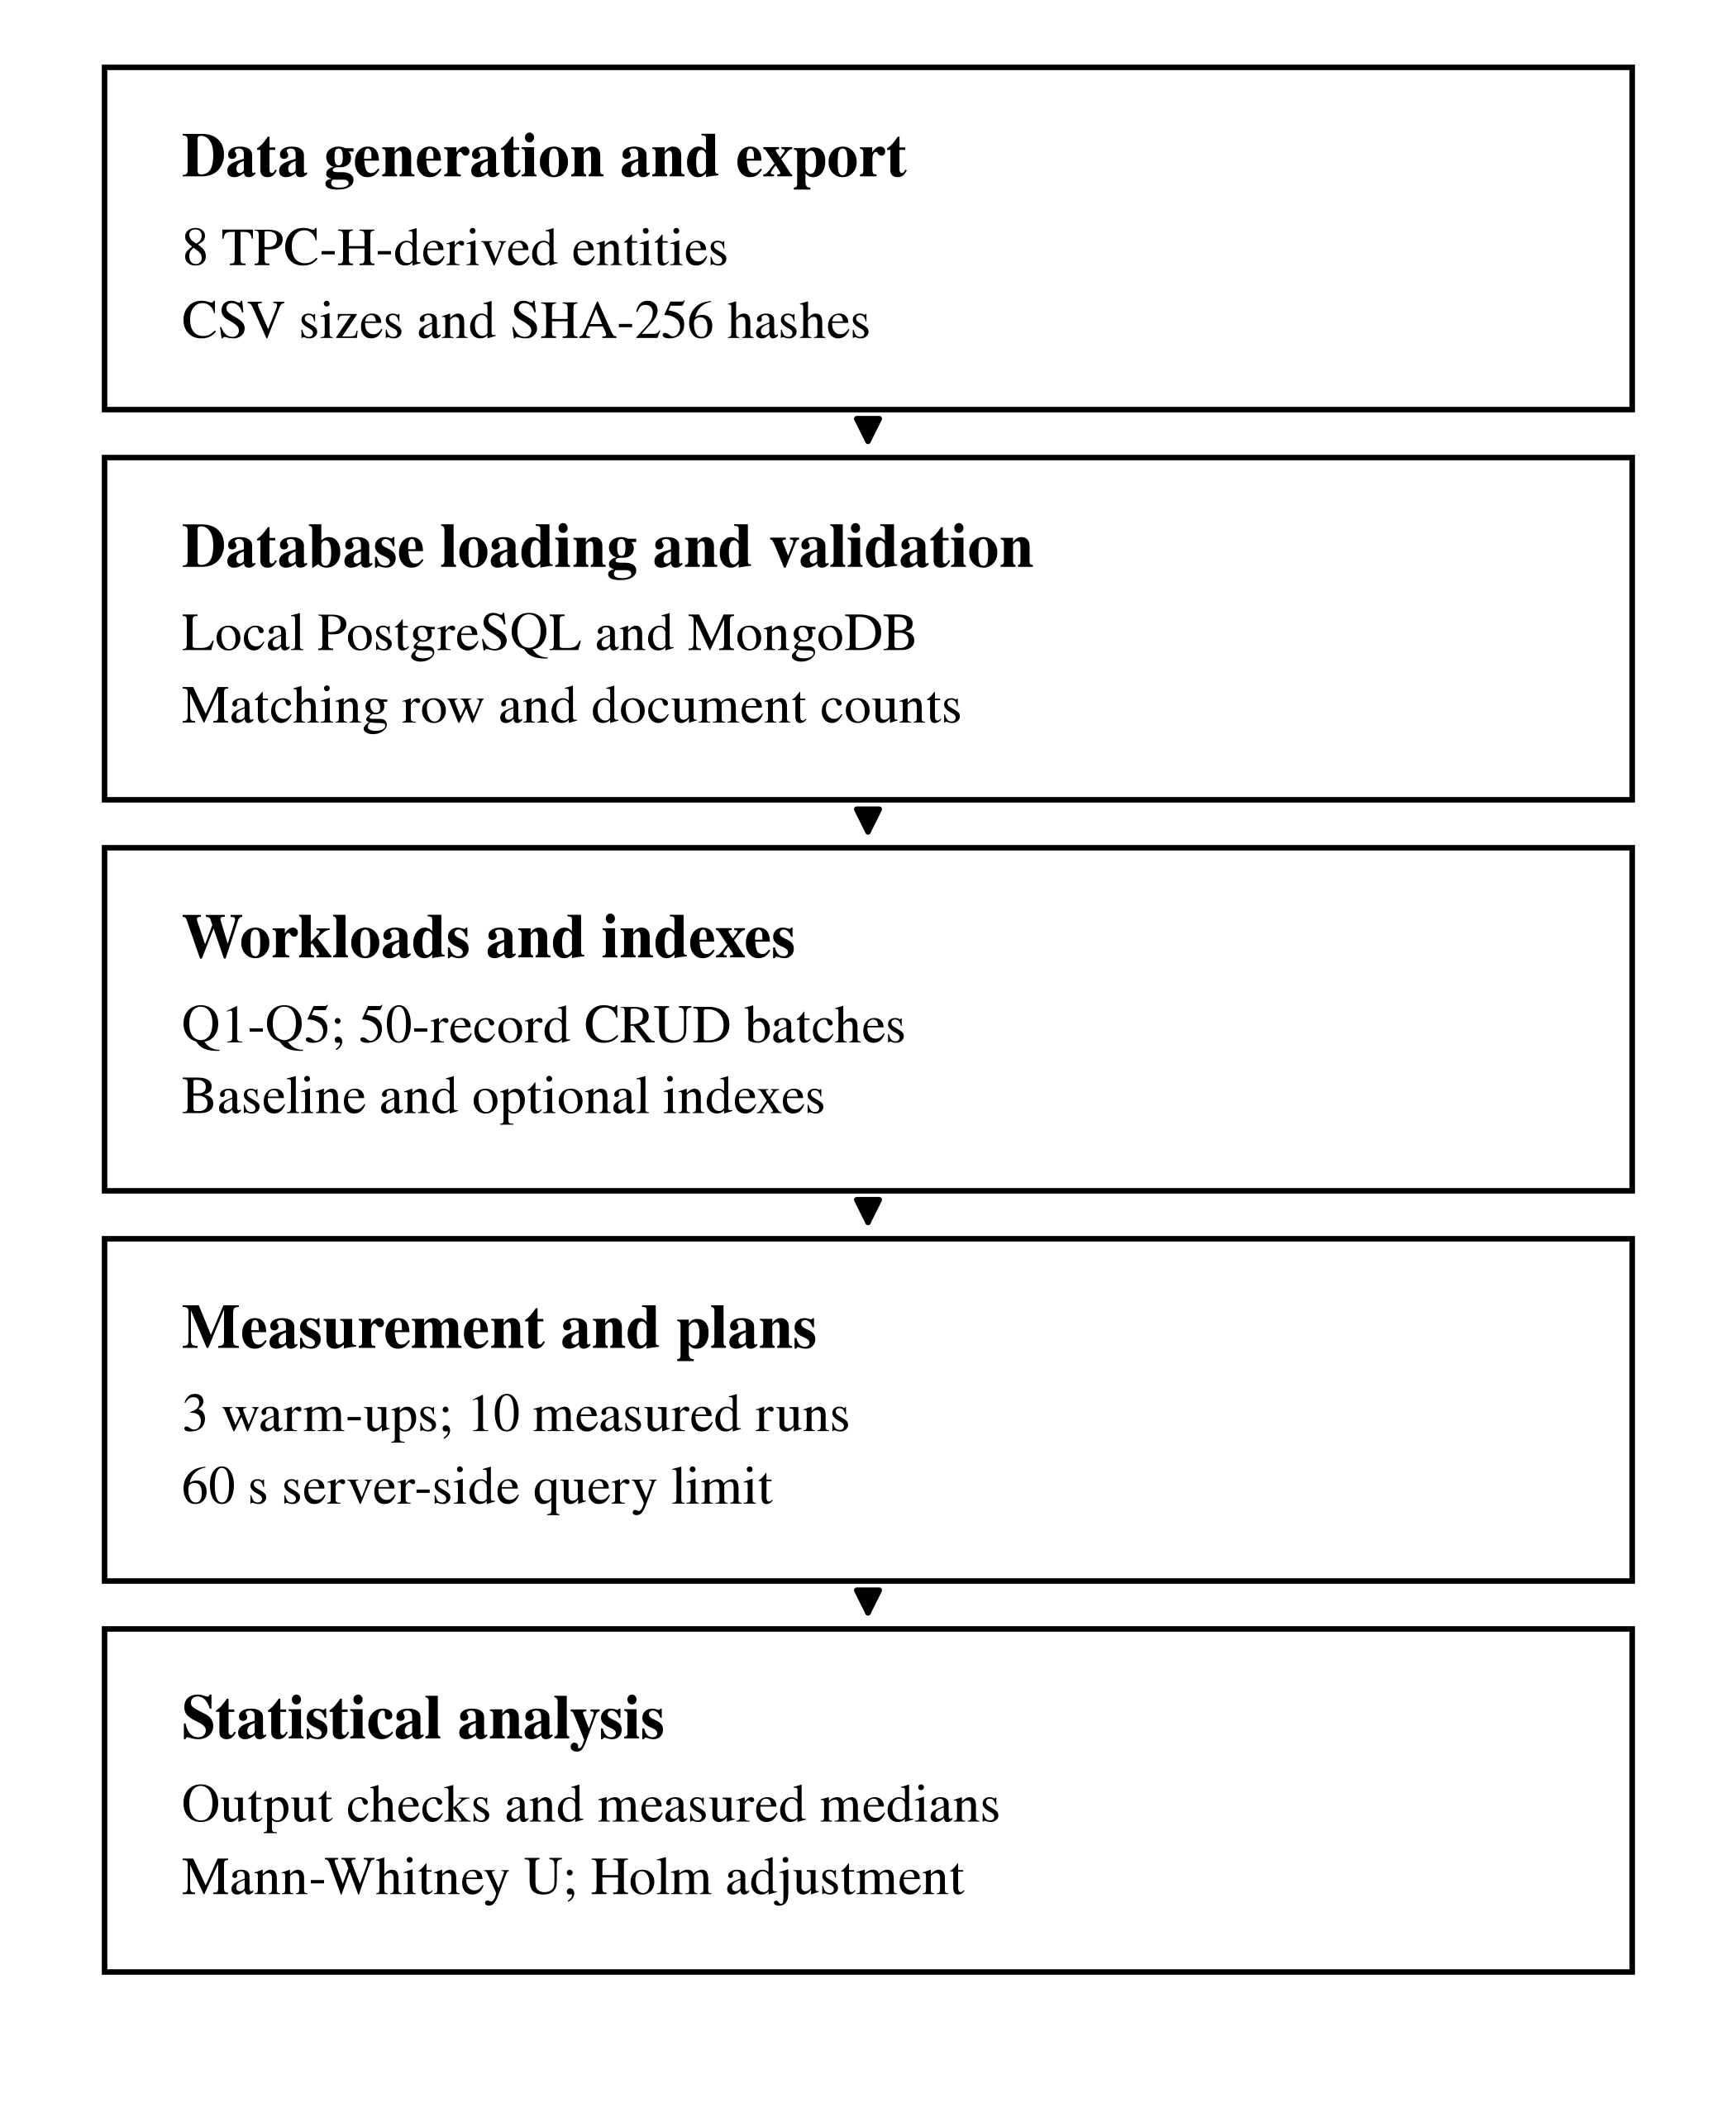
\includegraphics[width=\linewidth]{fig1_system_architecture.png}
  \caption{Five layers of the benchmark architecture. Data generation and loading precede query execution and measurement. Statistical analysis uses the recorded output.}
  \label{fig:arch}
\end{figure}

\subsection{MongoDB Implementation}
We created one collection for each of the eight TPC-H entities. Keeping related records in separate collections preserved the logical schema and removed denormalization as a source of variation in the comparison.

\subsection{PostgreSQL Architecture}
The PostgreSQL implementation uses eight normalized tables with declared primary and foreign keys. MongoDB stores corresponding entities in separate collections. Both baseline modes retain mandatory identifier indexes. In particular, PostgreSQL retains its primary-key indexes, whereas MongoDB retains its \texttt{\_id} indexes. The indexed mode adds the seven workload indexes defined in the repository on matching predicate and join fields. The baseline therefore means no optional workload indexes, rather than a complete absence of indexes.

\subsection{Data Consistency}
Figure~\ref{fig:datamodel} shows how the same entities were related in each database. In PostgreSQL, foreign keys enforce referential integrity along the \texttt{CUSTOMER}$\;\rightarrow\;$\texttt{ORDERS}$\;\rightarrow\;$\texttt{LINEITEM} chain. MongoDB links the corresponding collections when a query runs. Before taking measurements, we compared the row count in each table and the document count in each collection with the count in the source CSV file.

\begin{figure}[htbp]
  \centering
  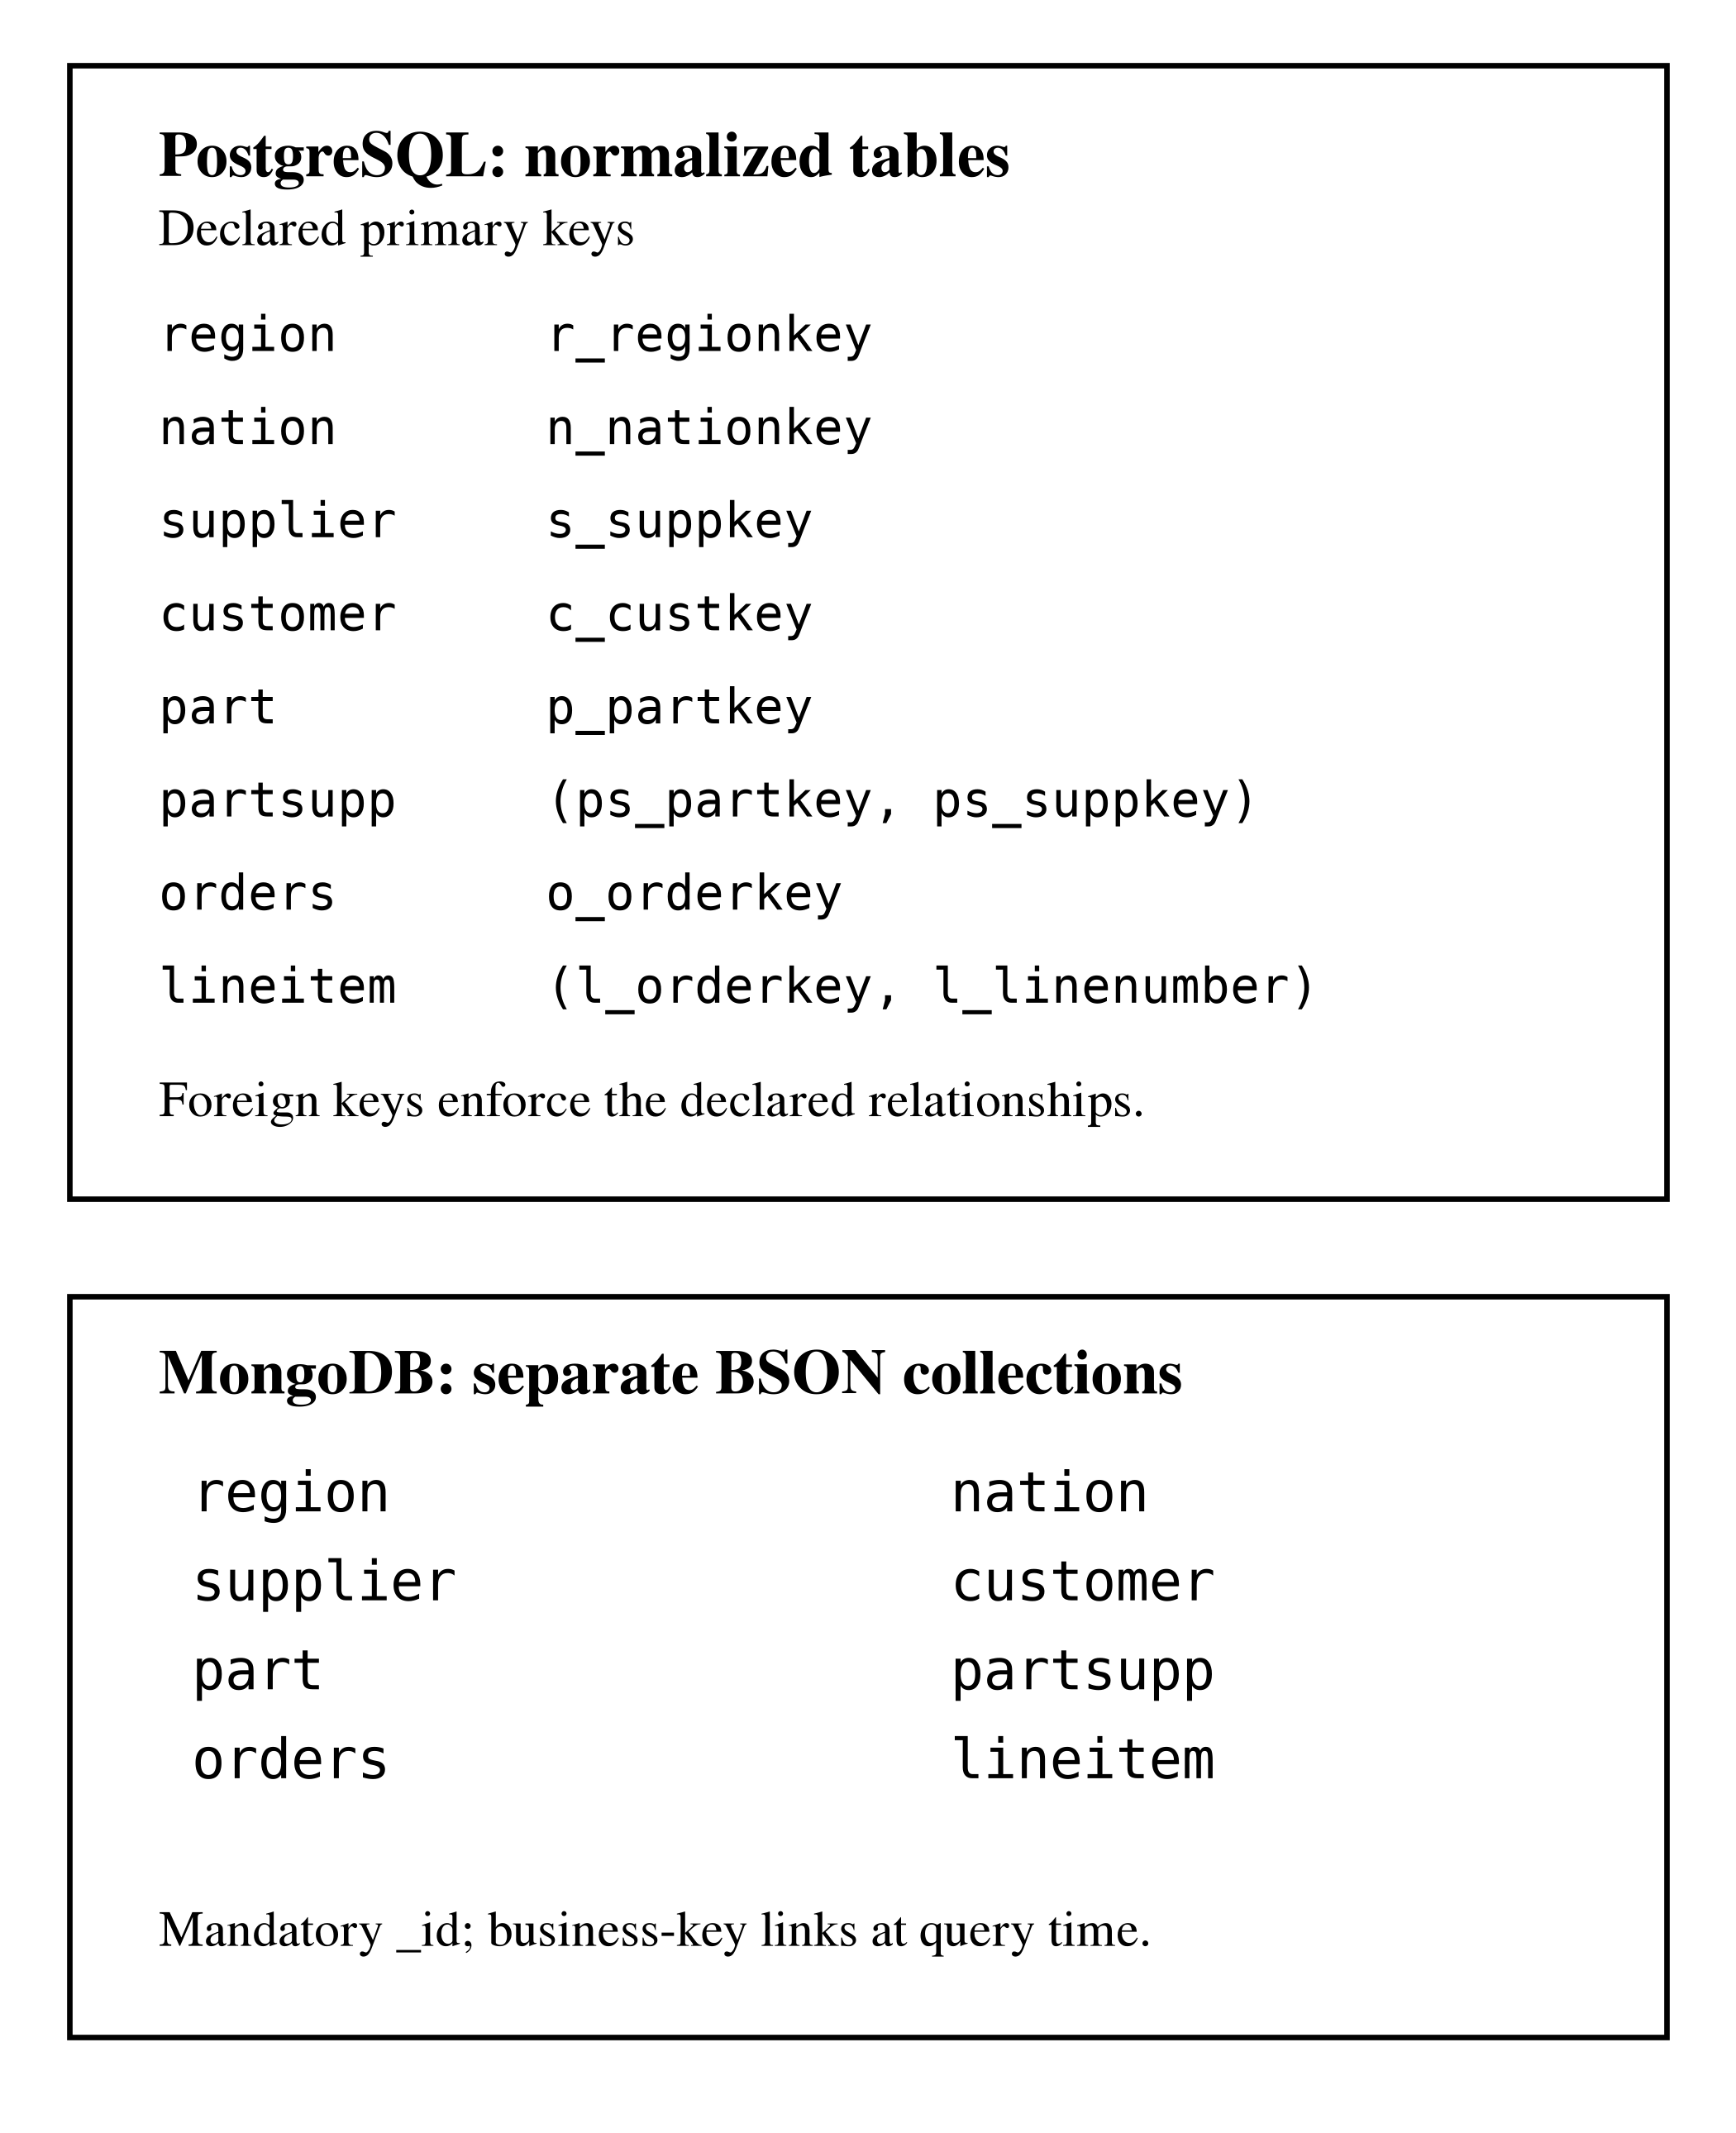
\includegraphics[width=\linewidth]{fig2_data_model_comparison.png}
  \caption{Logical schema in PostgreSQL and MongoDB. Each entity has a corresponding table and collection, so the comparison holds the choice of schema constant.}
  \label{fig:datamodel}
\end{figure}

% =====================================================================
\section{Experimental Methodology}
% =====================================================================

\subsection{CRUD Experiments}
Each completed configuration has three unmeasured warm-up runs followed by ten measured runs~\cite{raasveldt2018fair}. Engine order alternates between runs. CRUD trials operate on batches of 50 records. PostgreSQL bulk inserts use one \texttt{execute\_values} statement and MongoDB uses \texttt{insert\_many}. Reads issue 50 successive key lookups. Updates and deletes affect 50 records. Disposable insert/delete batches are restored before each trial, and updates start from the same account balance. Query timing ends after full result retrieval and client materialization. PostgreSQL rows are mapped to dictionaries, matching the MongoDB result representation. Canonicalization and multiset validation occur outside the timed interval. Both query/index configurations are measured before CRUD mutations. A server-side 60-second limit applies to each query. A timeout stops that engine\textquotesingle s remaining repetitions for that configuration and is reported as TO. Conditions without complete measurements are reported as NM.

\subsection{Query Experiments}
Table~\ref{tab:complexity} groups the queries by structural complexity and identifies the physical operators expected for each engine.

%% ── Table 2: Workload Complexity Matrix (spans both columns) ─────────
\begin{table*}[t]
\caption{Workload complexity and expected execution operators}
\label{tab:complexity}
\centering\small
\renewcommand{\arraystretch}{1.3}
\begin{adjustbox}{max width=\textwidth}
\begin{tabular}{@{}llcll@{}}
\toprule
\textbf{Workload} & \textbf{Query Type} & \textbf{Complexity Tier}
  & \textbf{MongoDB Expected Operator}
  & \textbf{PostgreSQL Expected Operator} \\ \midrule
$Q1$ & Equality Lookup    & Low      & \texttt{IXSCAN $\to$ FETCH}
     & \texttt{Index Scan} \\
$Q4$ & Two-way Join       & Moderate & \texttt{IXSCAN $\to$ \$lookup}
     & \texttt{Hash Join (Index Scan)} \\
$Q5$ & Join + Aggregation & High     & \texttt{\$lookup $\to$ \$match $\to$ \$group}
     & \texttt{Hash Join + HashAggregate} \\
\bottomrule
\end{tabular}
\end{adjustbox}
\end{table*}
%%─────────────────────────────────────────────────────────────────────

\subsubsection{Simple Queries}
$Q1$ (\emph{Equality lookup}) retrieves the customer with \texttt{c\_custkey=100}. PostgreSQL declares this field as a primary key. In MongoDB it is a business-key field distinct from \texttt{\_id}. It represents the low-complexity tier.

\subsubsection{Moderate Queries}
$Q4$ (\emph{Two-way join}) joins \texttt{CUSTOMER} to \texttt{ORDERS} on an equality condition and represents the moderate-complexity tier.

\subsubsection{Complex Queries}
$Q5$ (\emph{Join + aggregation}) represents the high-complexity tier. It joins \texttt{ORDERS} and \texttt{LINEITEM} on the order key, filters ship dates from 1994-01-01 inclusive to 1995-01-01 exclusive, groups by order priority, computes a count and the sum of extended price multiplied by one minus discount, and sorts by revenue. The implementation contains one join between two entities. MongoDB uses numeric doubles and PostgreSQL uses exact numeric values. Aggregate output validation rounds revenue to four decimal places.

% =====================================================================
\section{Performance Measurements}
% =====================================================================

\subsection{Insert Throughput}
We calculated throughput for each measured 50-record insert batch as
\begin{equation}
  \text{Throughput} = \frac{N_{\text{ops}}}{T_{\text{total}}}
  \label{eq:throughput}
\end{equation}
where $N_{\text{ops}}=50$ is the number of acknowledged records and $T_{\text{total}}$ is the batch wall-clock time. Figure~\ref{fig:insert} reports the observed medians. The comparison uses loopback connections and each deployment\textquotesingle s stated write acknowledgment. At SF~1.0 with optional indexes, the median insert-batch latency was 5.68\,ms for MongoDB and 2.84\,ms for PostgreSQL. Their respective throughputs were 8{,}817 and 17{,}591 records/s, corresponding to a reported $2.00\times$ PostgreSQL speedup.

\begin{figure}[htbp]
  \centering
  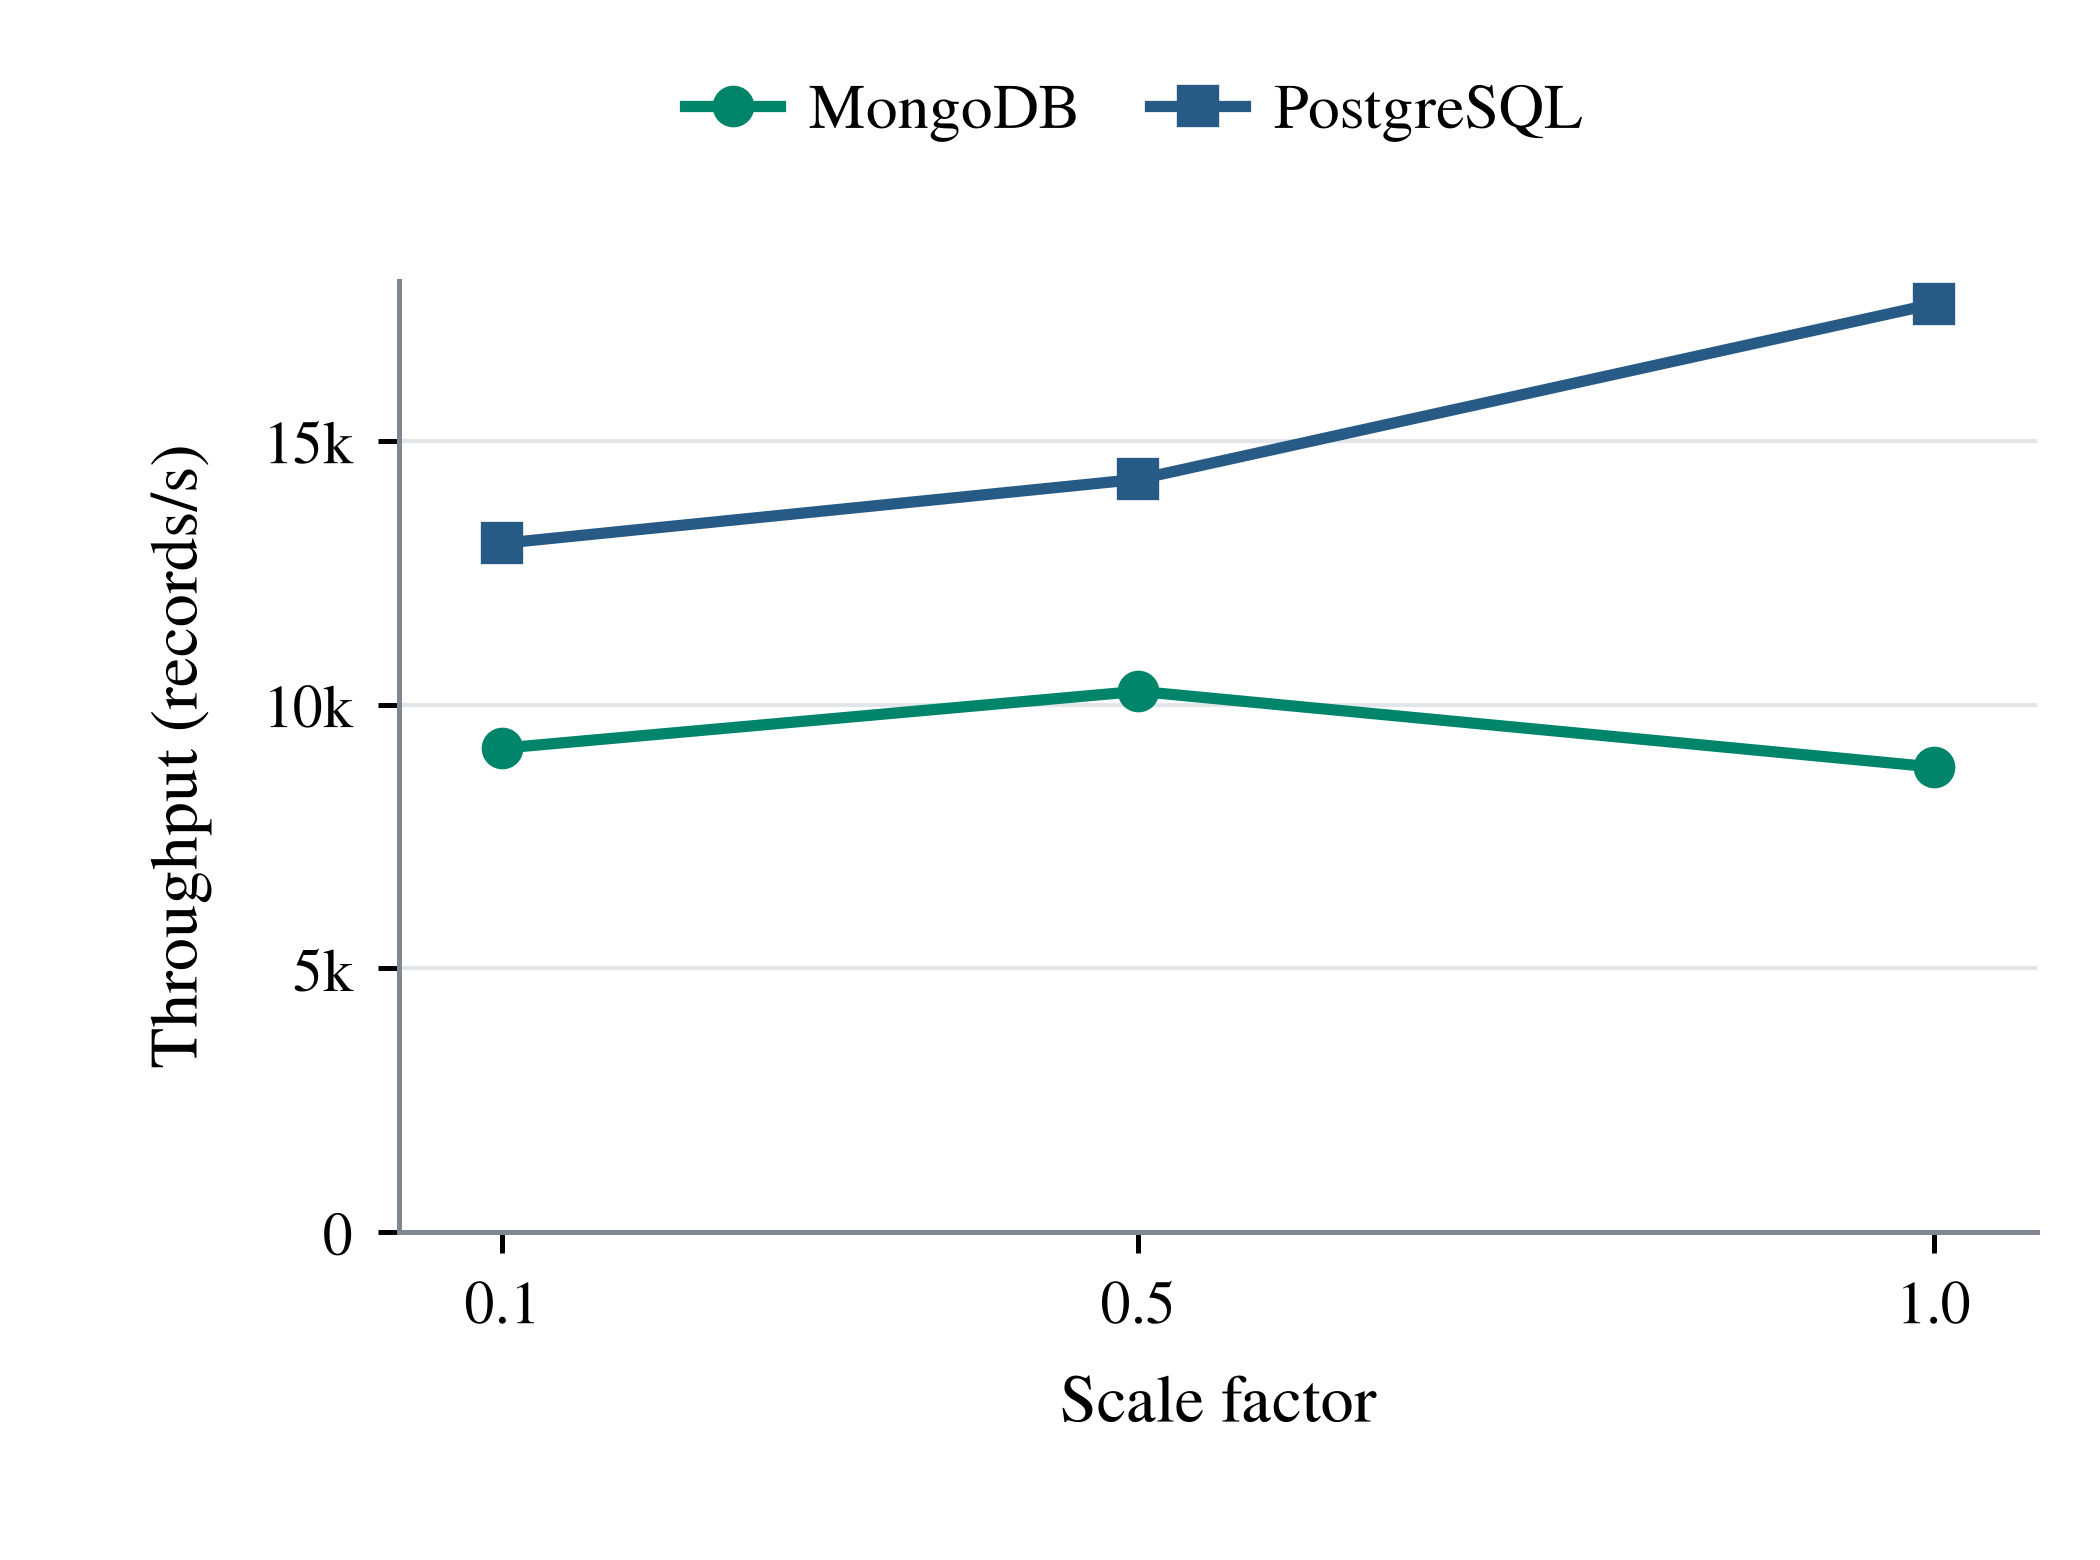
\includegraphics[width=\linewidth]{fig4_insert_throughput.png}
  \caption{Median throughput of acknowledged 50-record insert batches with optional indexes enabled.}
  \label{fig:insert}
\end{figure}

\subsection{Update Performance}
Update trials add 10.00 to the account balances of 50 customers after restoring their starting values. The measured batch medians are reported in Figure~\ref{fig:crud}. The measurements determine the scaling pattern. A linear relation is not assumed. For indexed SF~1.0, median update-batch latency was 3.40\,ms for MongoDB and 0.84\,ms for PostgreSQL, with respective throughputs of 14{,}725 and 59{,}690 records/s and a reported $4.05\times$ PostgreSQL speedup.

\subsection{Delete Performance}
Each delete trial removes a freshly restored disposable batch of 50 customers. Figure~\ref{fig:crud} reports its measured latency. The results do not identify a causal role for reclamation or checkpointing because these background activities were not profiled. At indexed SF~1.0, median delete-batch latency was 6.03\,ms for MongoDB and 1.94\,ms for PostgreSQL, with respective throughputs of 8{,}286 and 25{,}790 records/s and a reported $3.11\times$ PostgreSQL speedup. Without optional indexes at the same scale, MongoDB recorded 208.05\,ms and 240 records/s, compared with 13{,}173.75\,ms and 3.8 records/s for PostgreSQL, a reported $63.32\times$ MongoDB speedup.

\begin{figure}[htbp]
  \centering
  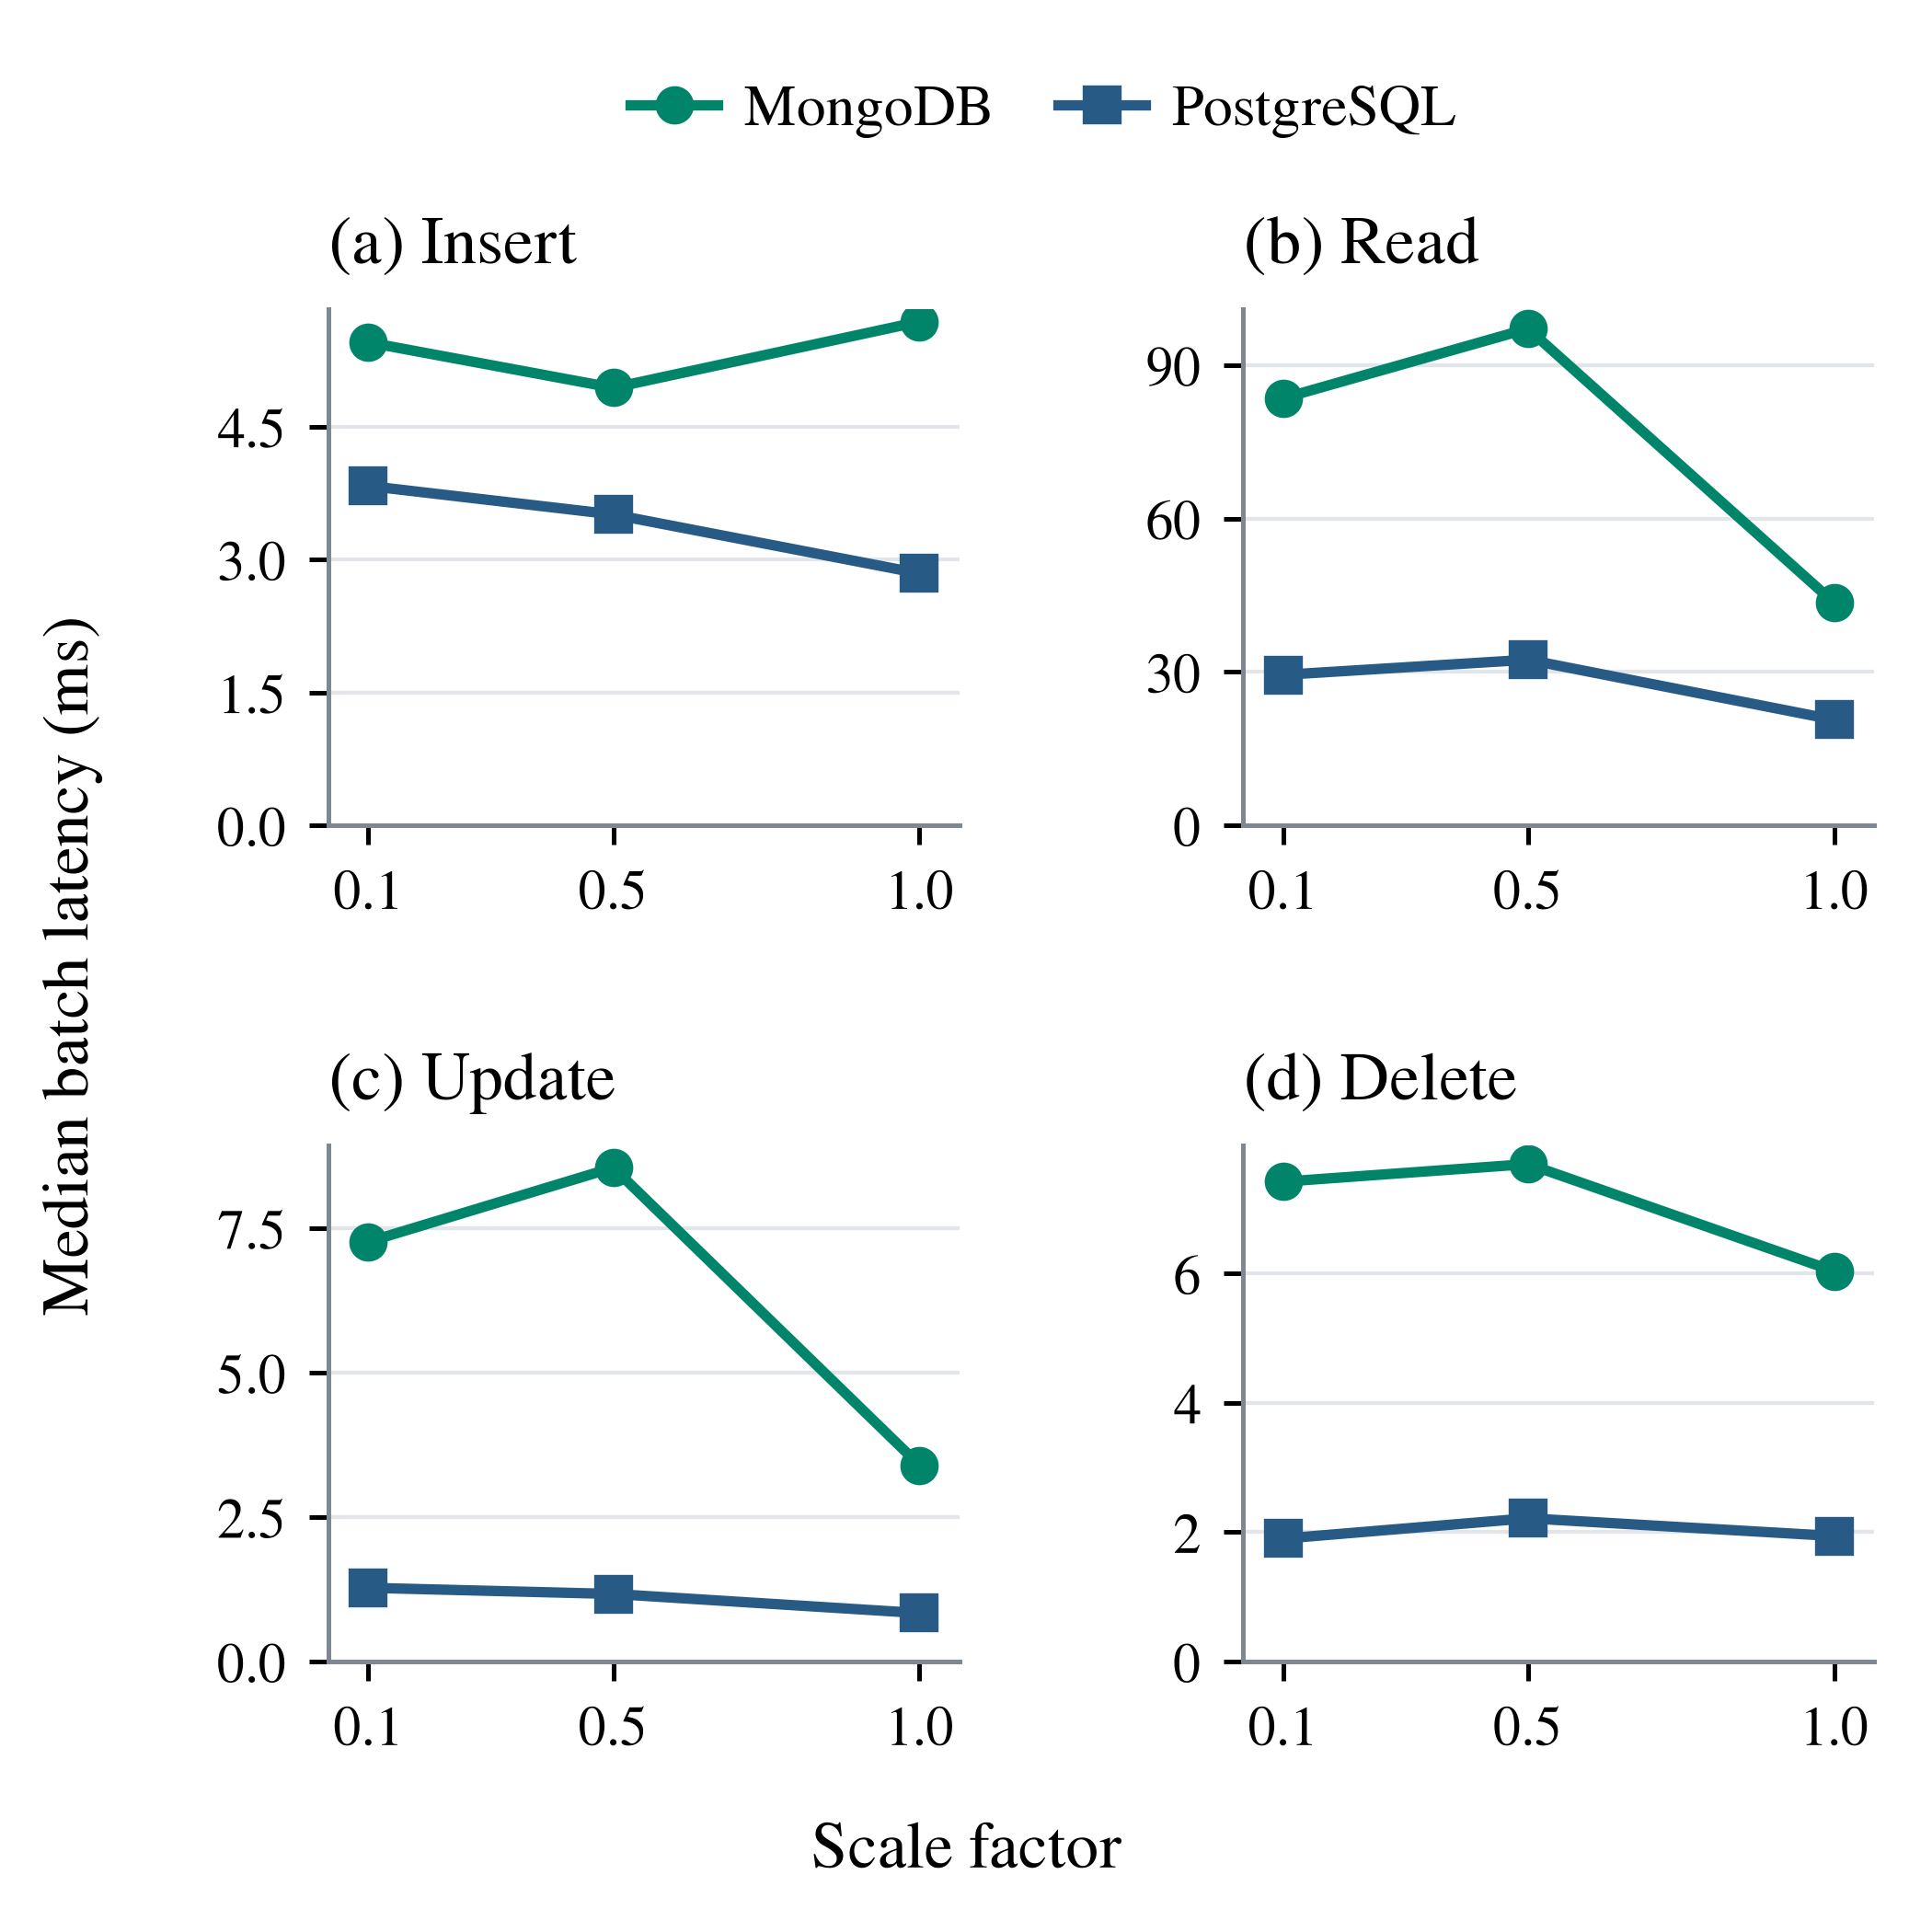
\includegraphics[width=\linewidth]{fig3_crud_latency.png}
  \caption{Median latency of indexed 50-record CRUD batches. Reads use successive key lookups. Each write trial begins from its restored state.}
  \label{fig:crud}
\end{figure}

\subsection{Query Response Time}
We measured latency at the client as
\begin{equation}
  L = t_{\text{end}} - t_{\text{start}}
  \label{eq:latency}
\end{equation}
where $t_{\text{start}}$ is recorded immediately before query submission and $t_{\text{end}}$ after receipt of the final result. Figure~\ref{fig:latvol} reports the median of each complete ten-run configuration. Both database servers ran on the same Windows host over loopback connections. The results characterize the recorded single-node settings, derived datasets, and warm-cache workloads.

\begin{figure}[htbp]
  \centering
  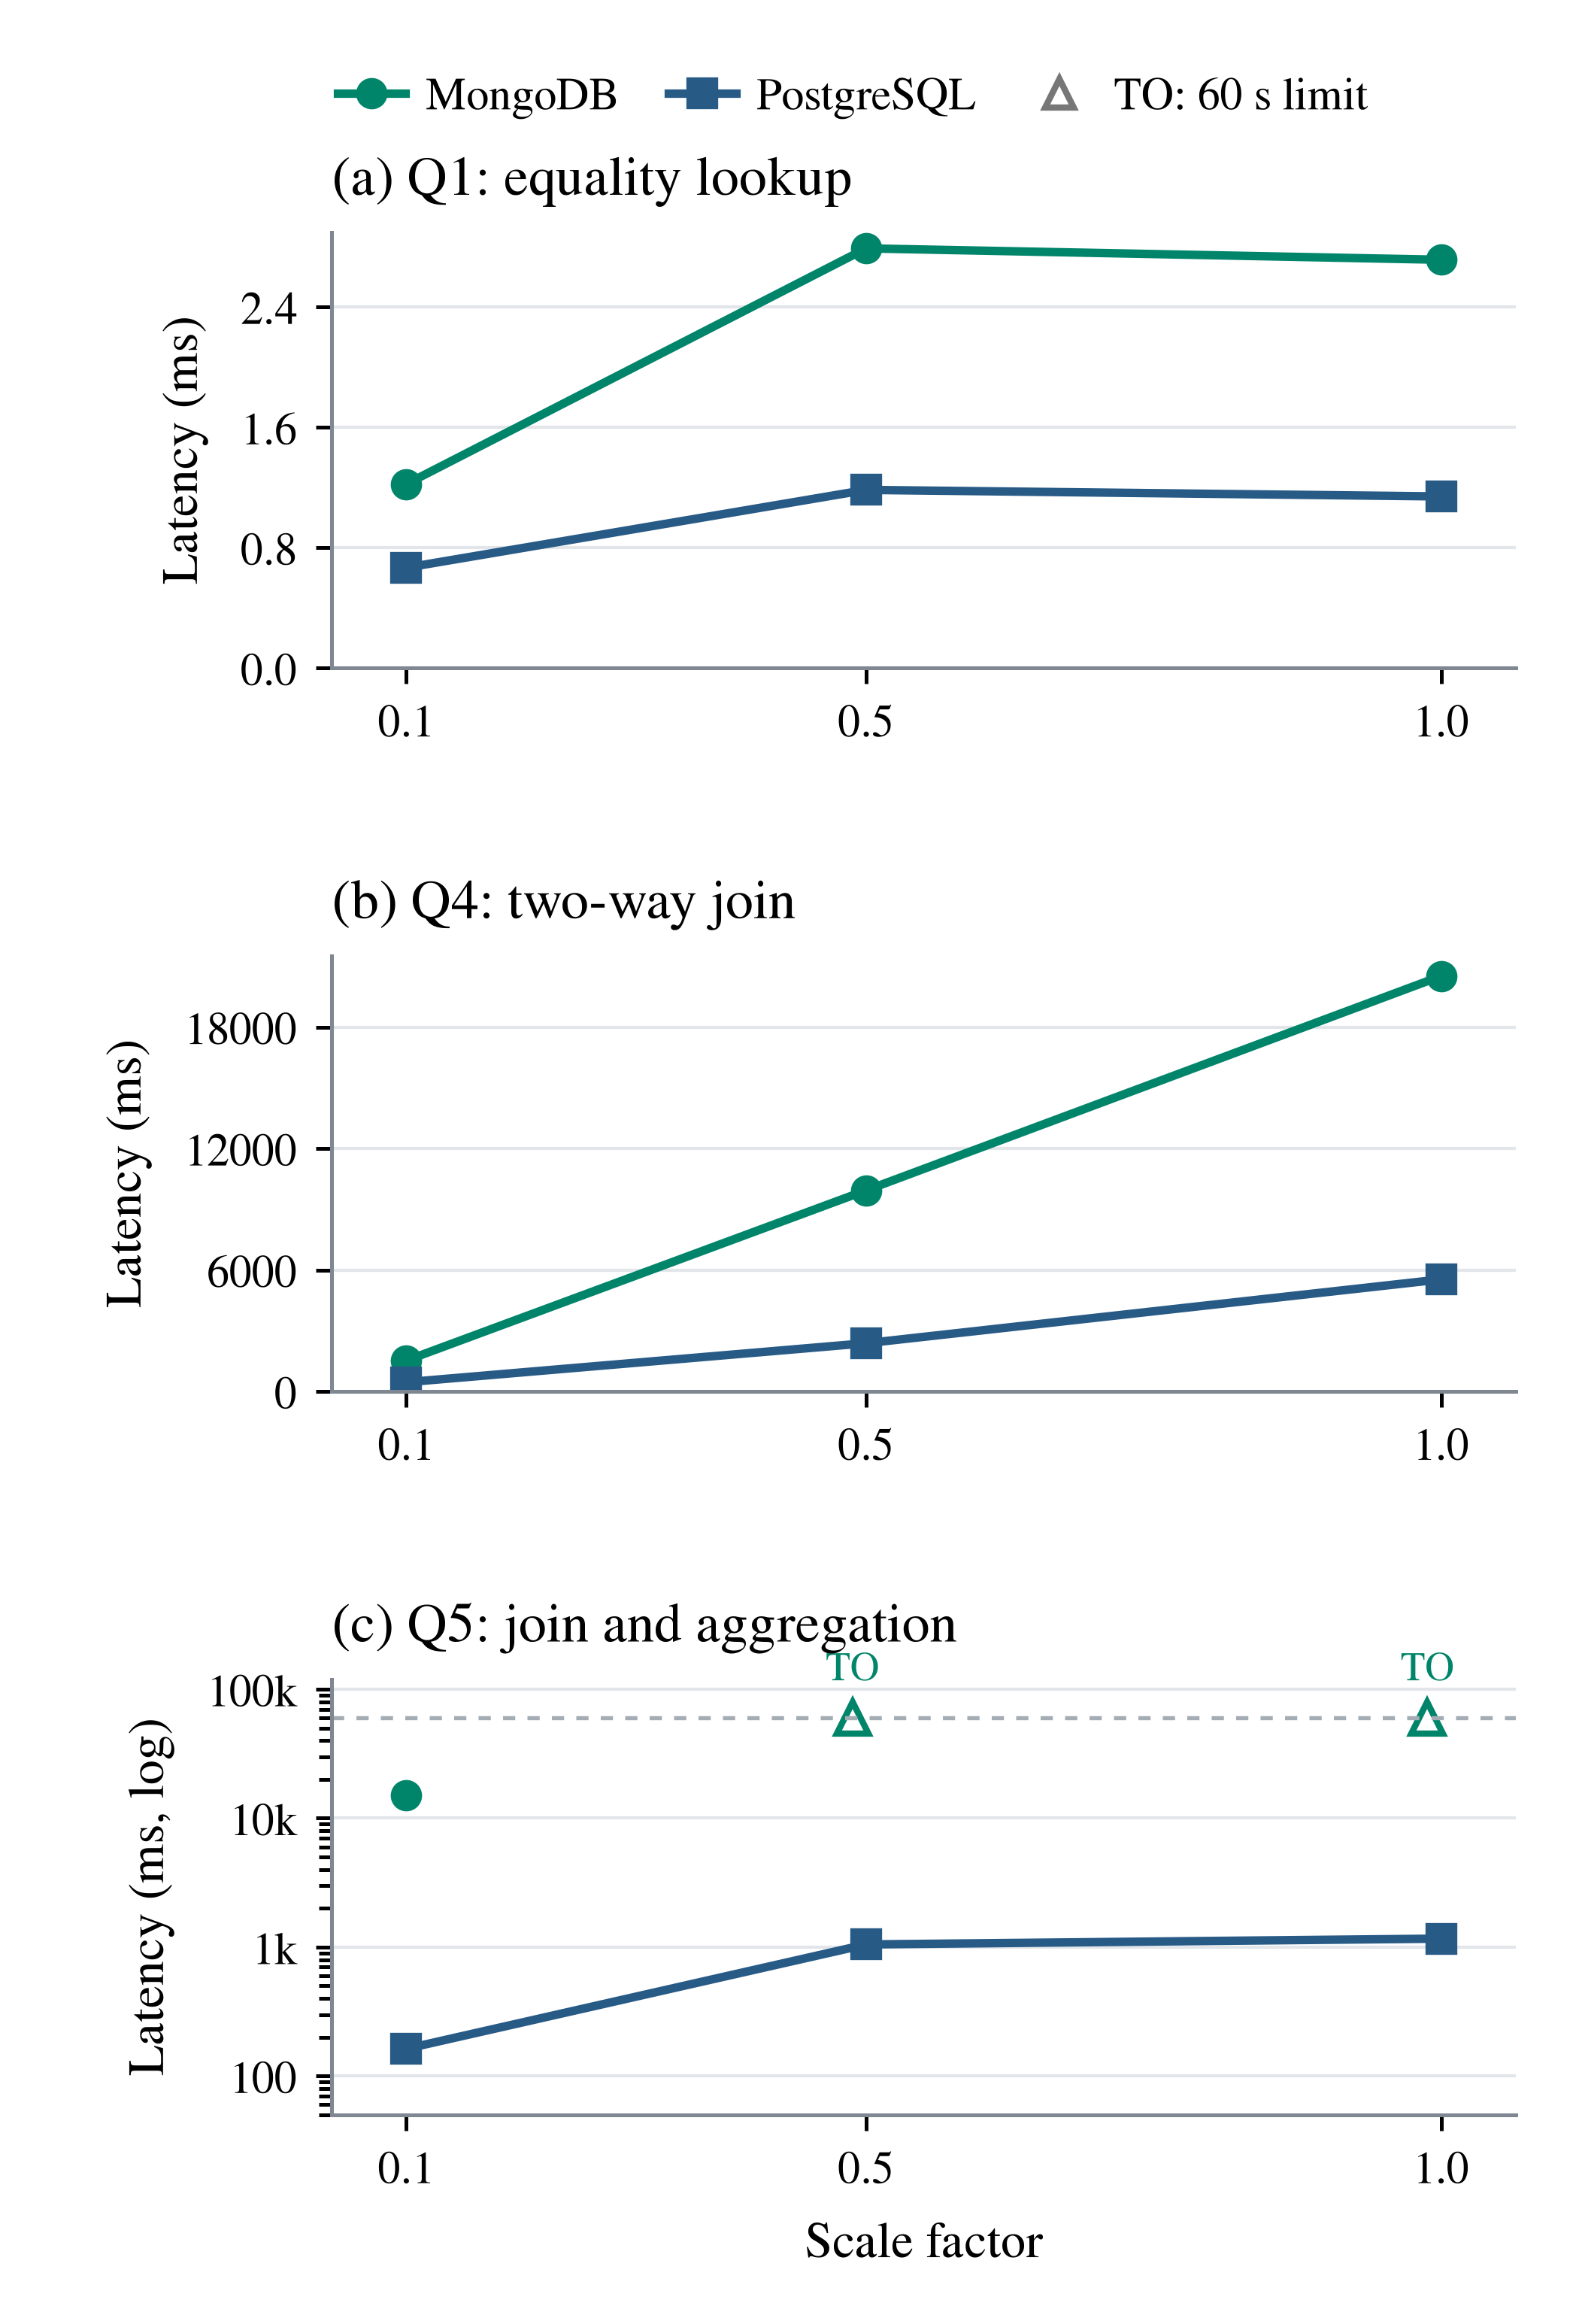
\includegraphics[width=\linewidth]{fig7_latency_vs_volume.png}
  \caption{Median indexed-query latency by scale factor. TO marks the 60-second server limit and is not a measured median.}
  \label{fig:latvol}
\end{figure}

\subsection{Storage Overhead}
We measured the space allocated on disk to base data and B-tree indexes. The storage overhead ratio was
\begin{equation}
  \rho = \frac{S_{\text{DB}}}{S_{\text{raw}}}
  \label{eq:storage}
\end{equation}
where $S_{\text{DB}}$ is the total on-disk footprint (data plus indexes) and $S_{\text{raw}}$
is the size of the original CSV dataset.

% =====================================================================
\section{Analysis}
% =====================================================================

\subsection{Effect of Data Volume}
Figure~\ref{fig:q1lookup} reports measured $Q1$ medians. Figure~\ref{fig:rangemulti} reports $Q2$ and $Q3$ with the fixed repository predicates. Their result counts are retained in the evidence, including zero-result cases. These observations do not constitute a controlled sweep of predicate selectivity.

\subsubsection{Small (SF\,=\,0.1)}
For indexed $Q1$, the median latency was 1.22\,ms for MongoDB and 0.67\,ms for PostgreSQL.

\subsubsection{Moderate (SF\,=\,0.5)}
For indexed $Q1$, the median latency was 2.79\,ms for MongoDB and 1.18\,ms for PostgreSQL.

\subsubsection{Large (SF\,=\,1.0)}
For indexed $Q1$, the median latency was 2.71\,ms for MongoDB and 1.14\,ms for PostgreSQL.

\begin{figure}[htbp]
  \centering
  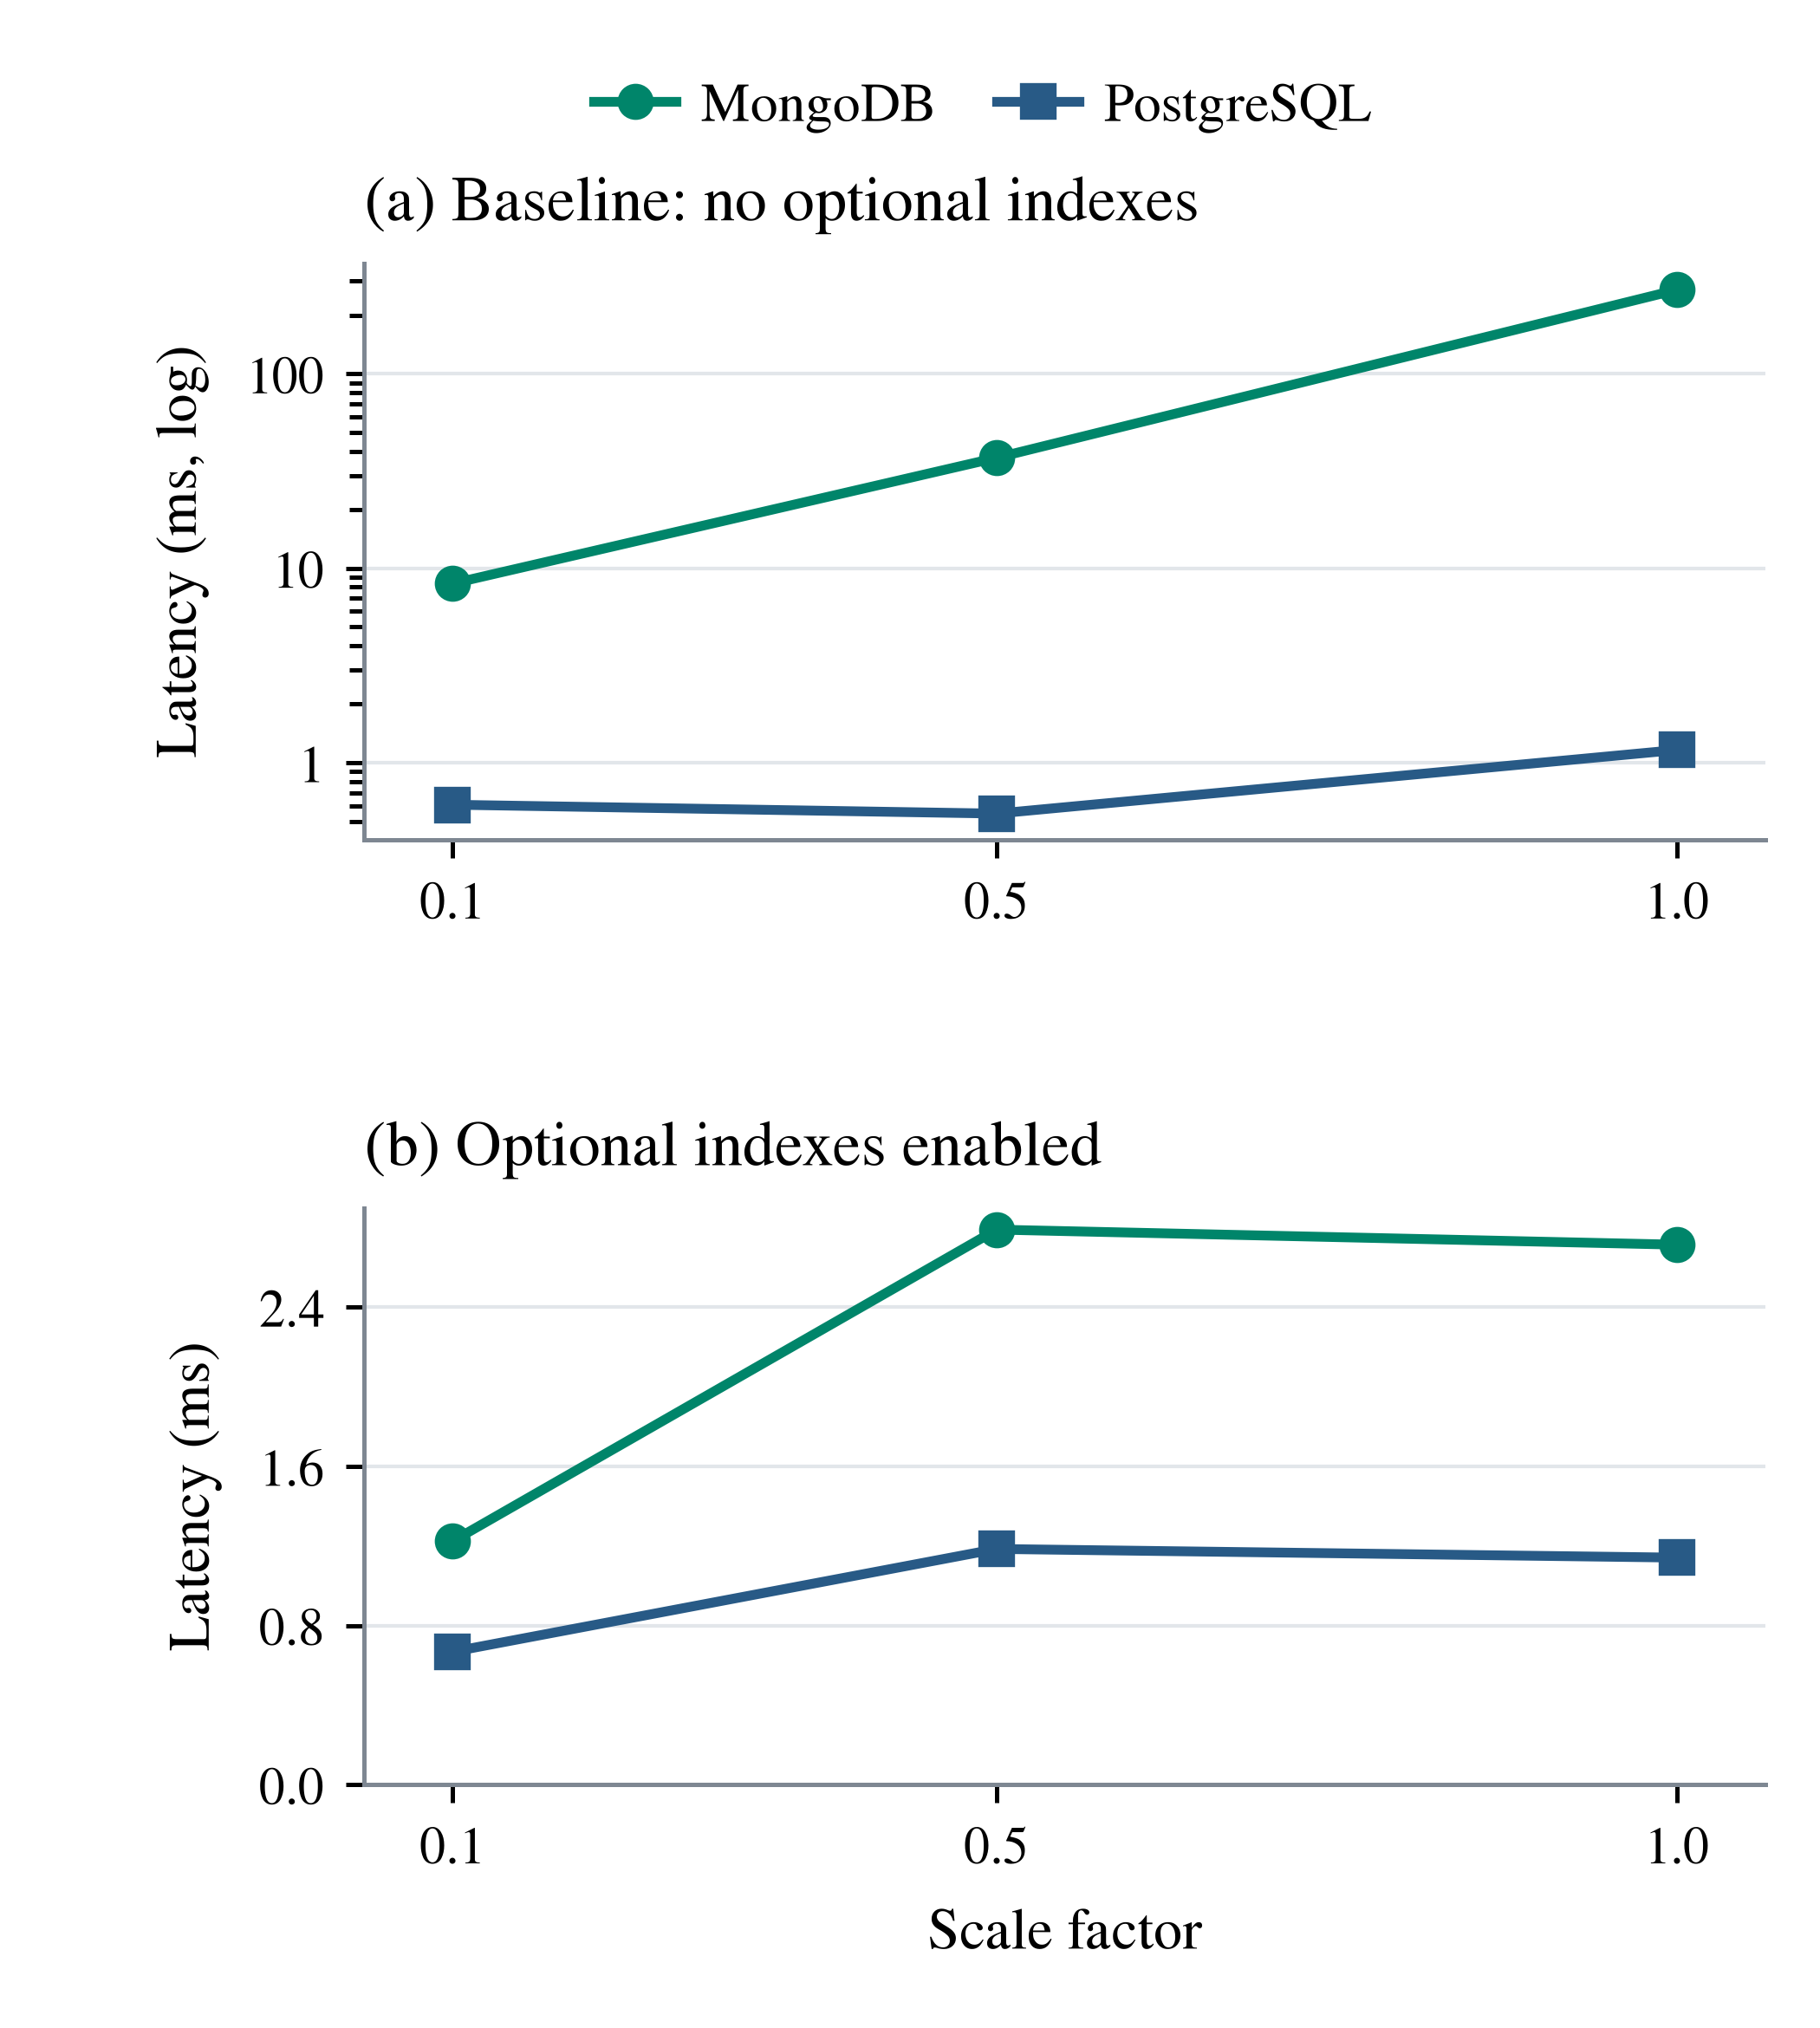
\includegraphics[width=\linewidth]{fig5_q1_lookup_latency.png}
  \caption{Measured equality-lookup medians by data volume and index configuration. The baseline retains PostgreSQL primary-key indexes and MongoDB identifier indexes.}
  \label{fig:q1lookup}
\end{figure}

\begin{figure}[htbp]
  \centering
  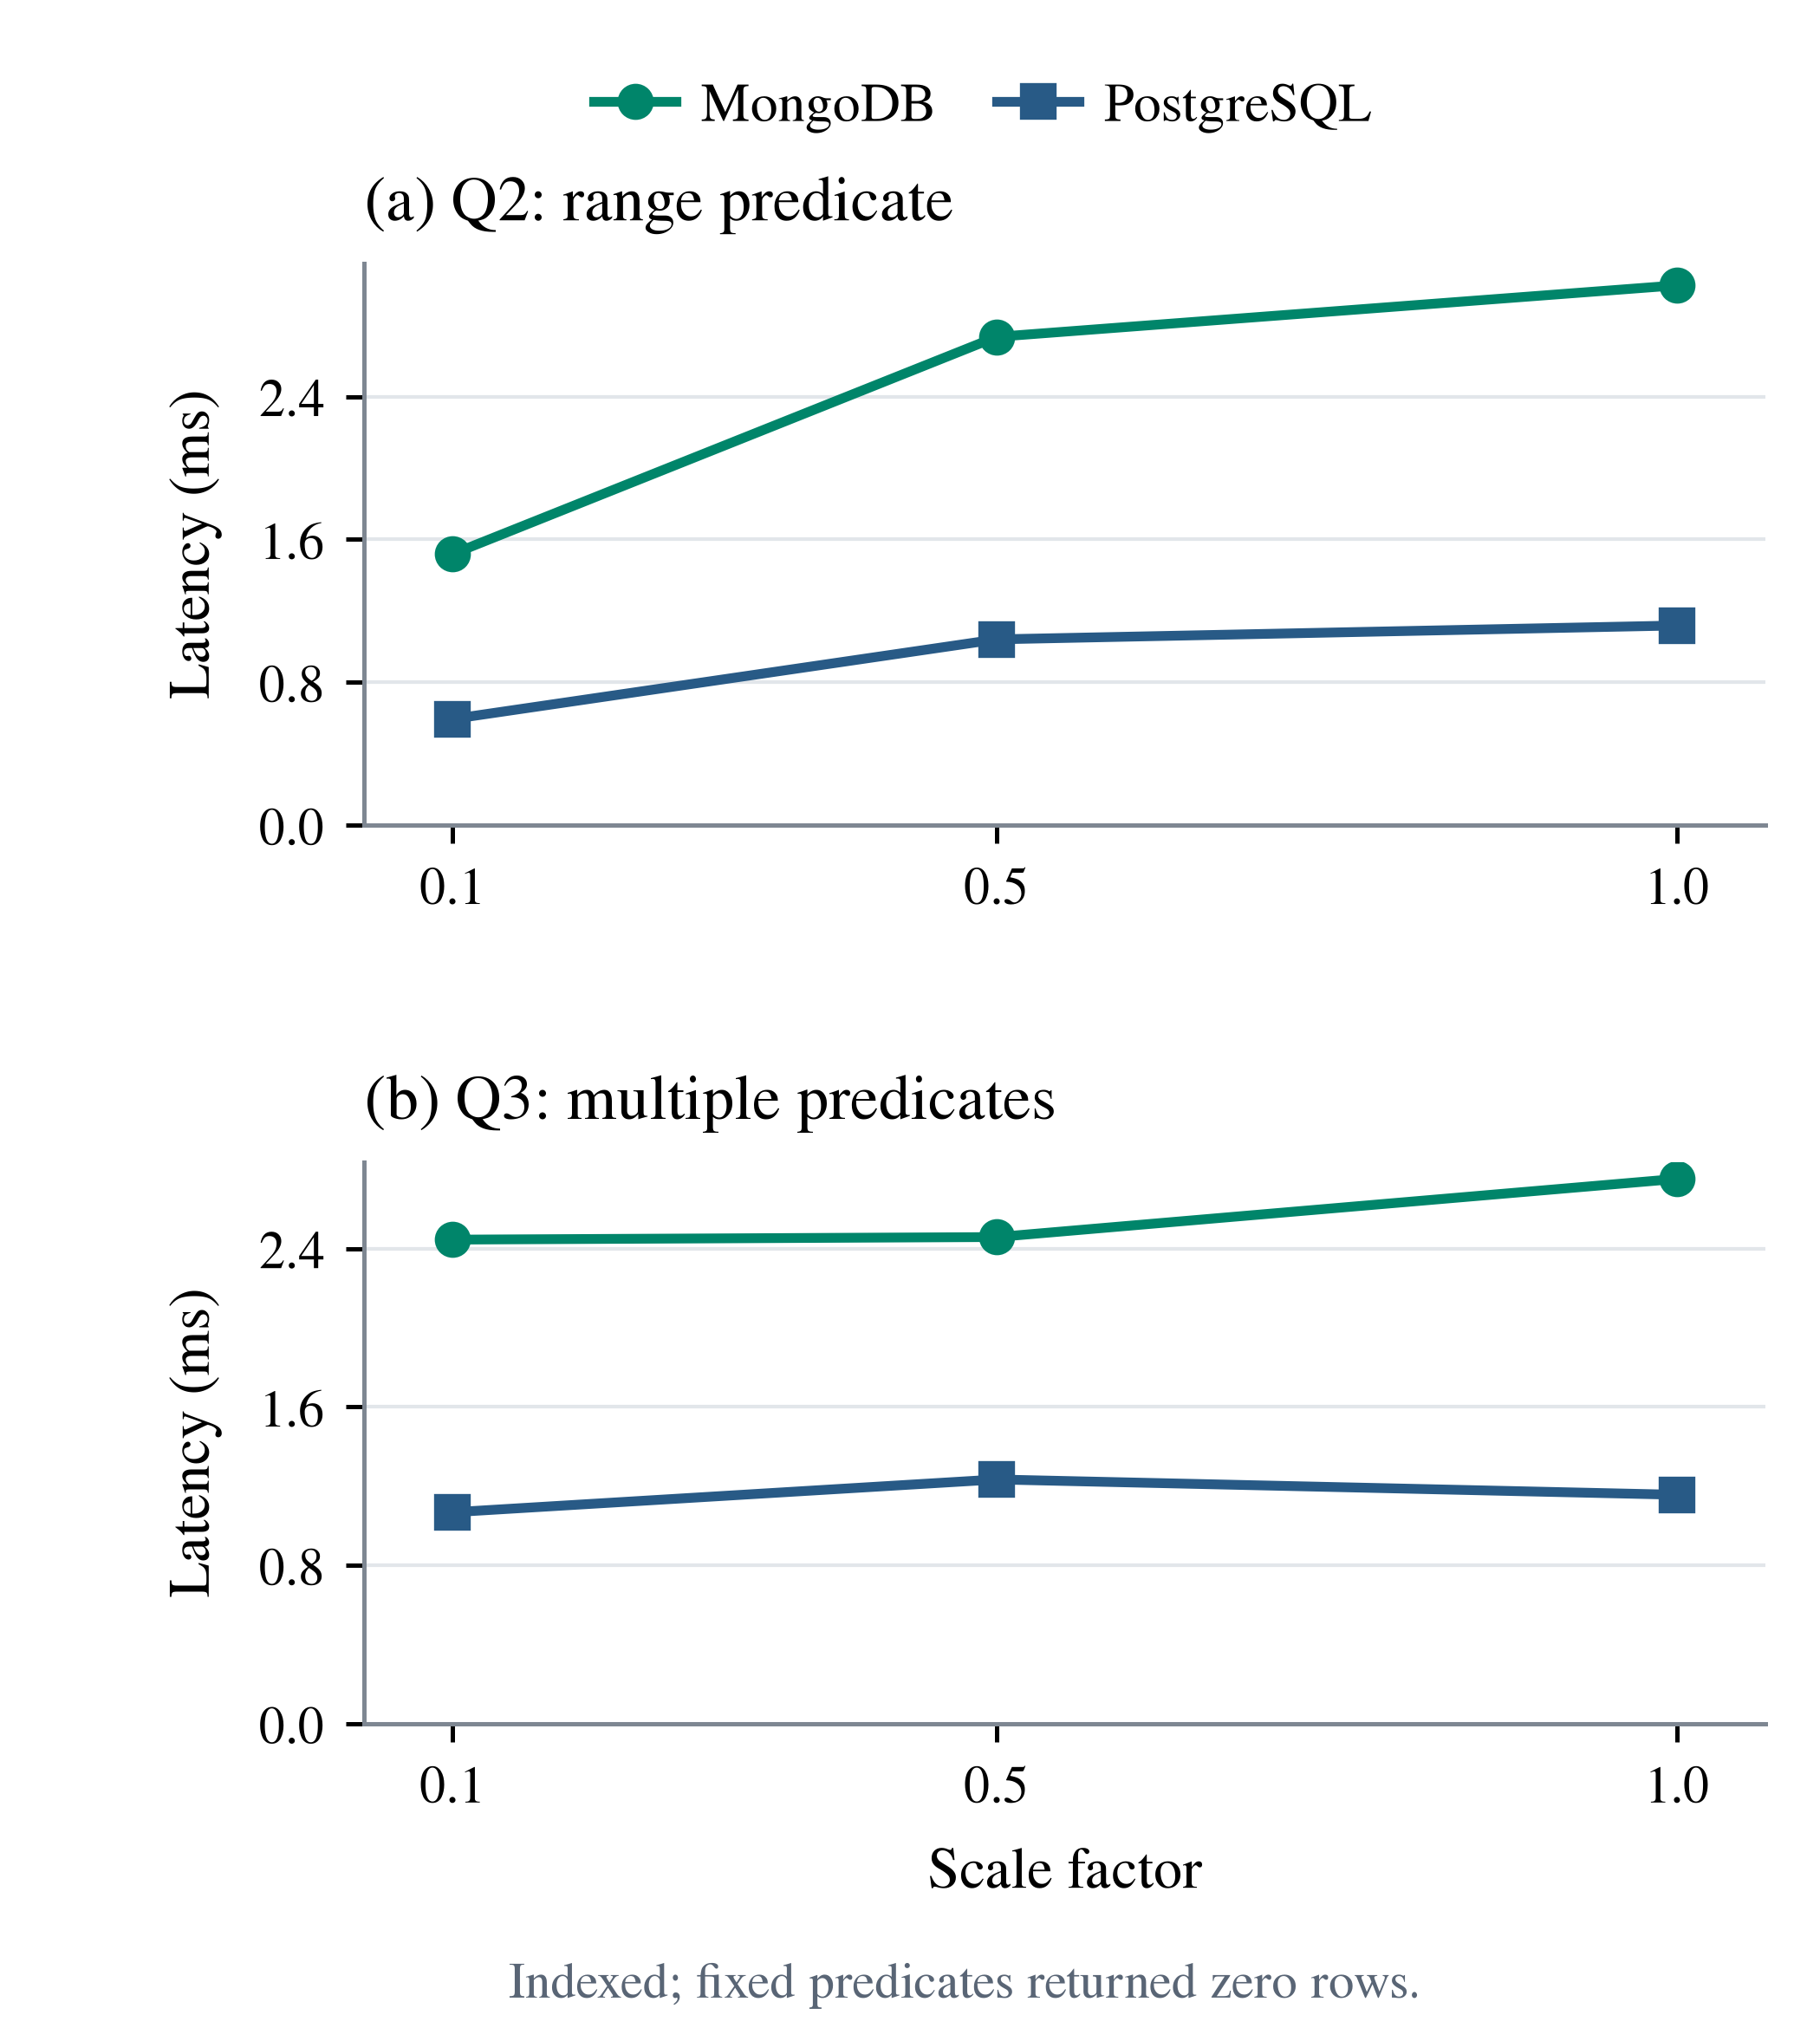
\includegraphics[width=\linewidth]{fig6_range_multi_latency.png}
  \caption{Indexed range and multi-condition query latency with the fixed repository predicates. Both queries returned zero rows in the recorded conditions.}
  \label{fig:rangemulti}
\end{figure}

\subsection{Effect of Query Complexity}
Figure~\ref{fig:complexity} compares the measured $Q1$, $Q4$, and $Q5$ medians at SF~1.0. Figure~\ref{fig:joinagg} reports join and aggregation latency at all scales. Executed plans, rather than query syntax alone, identify the physical join strategies. The comparison does not assume that every MongoDB \texttt{\$lookup} uses a nested loop or that PostgreSQL always selects a hash join.

\subsubsection{Simple}
An indexed equality lookup can use the relevant business-key index. PostgreSQL can also use its retained primary-key index in the baseline mode.

\subsubsection{Moderate}
The two-way join combines customers in the BUILDING market segment with their orders. Both engines return the same five projected fields. This avoids the larger nested payload returned by the original MongoDB pipeline.

\subsubsection{Complex}
Grouping and sorting may require intermediate state in both engines. The saved executed plans identify the chosen operators. Latency alone does not establish the memory cost or the reason for a difference between engines.

\begin{figure}[htbp]
  \centering
  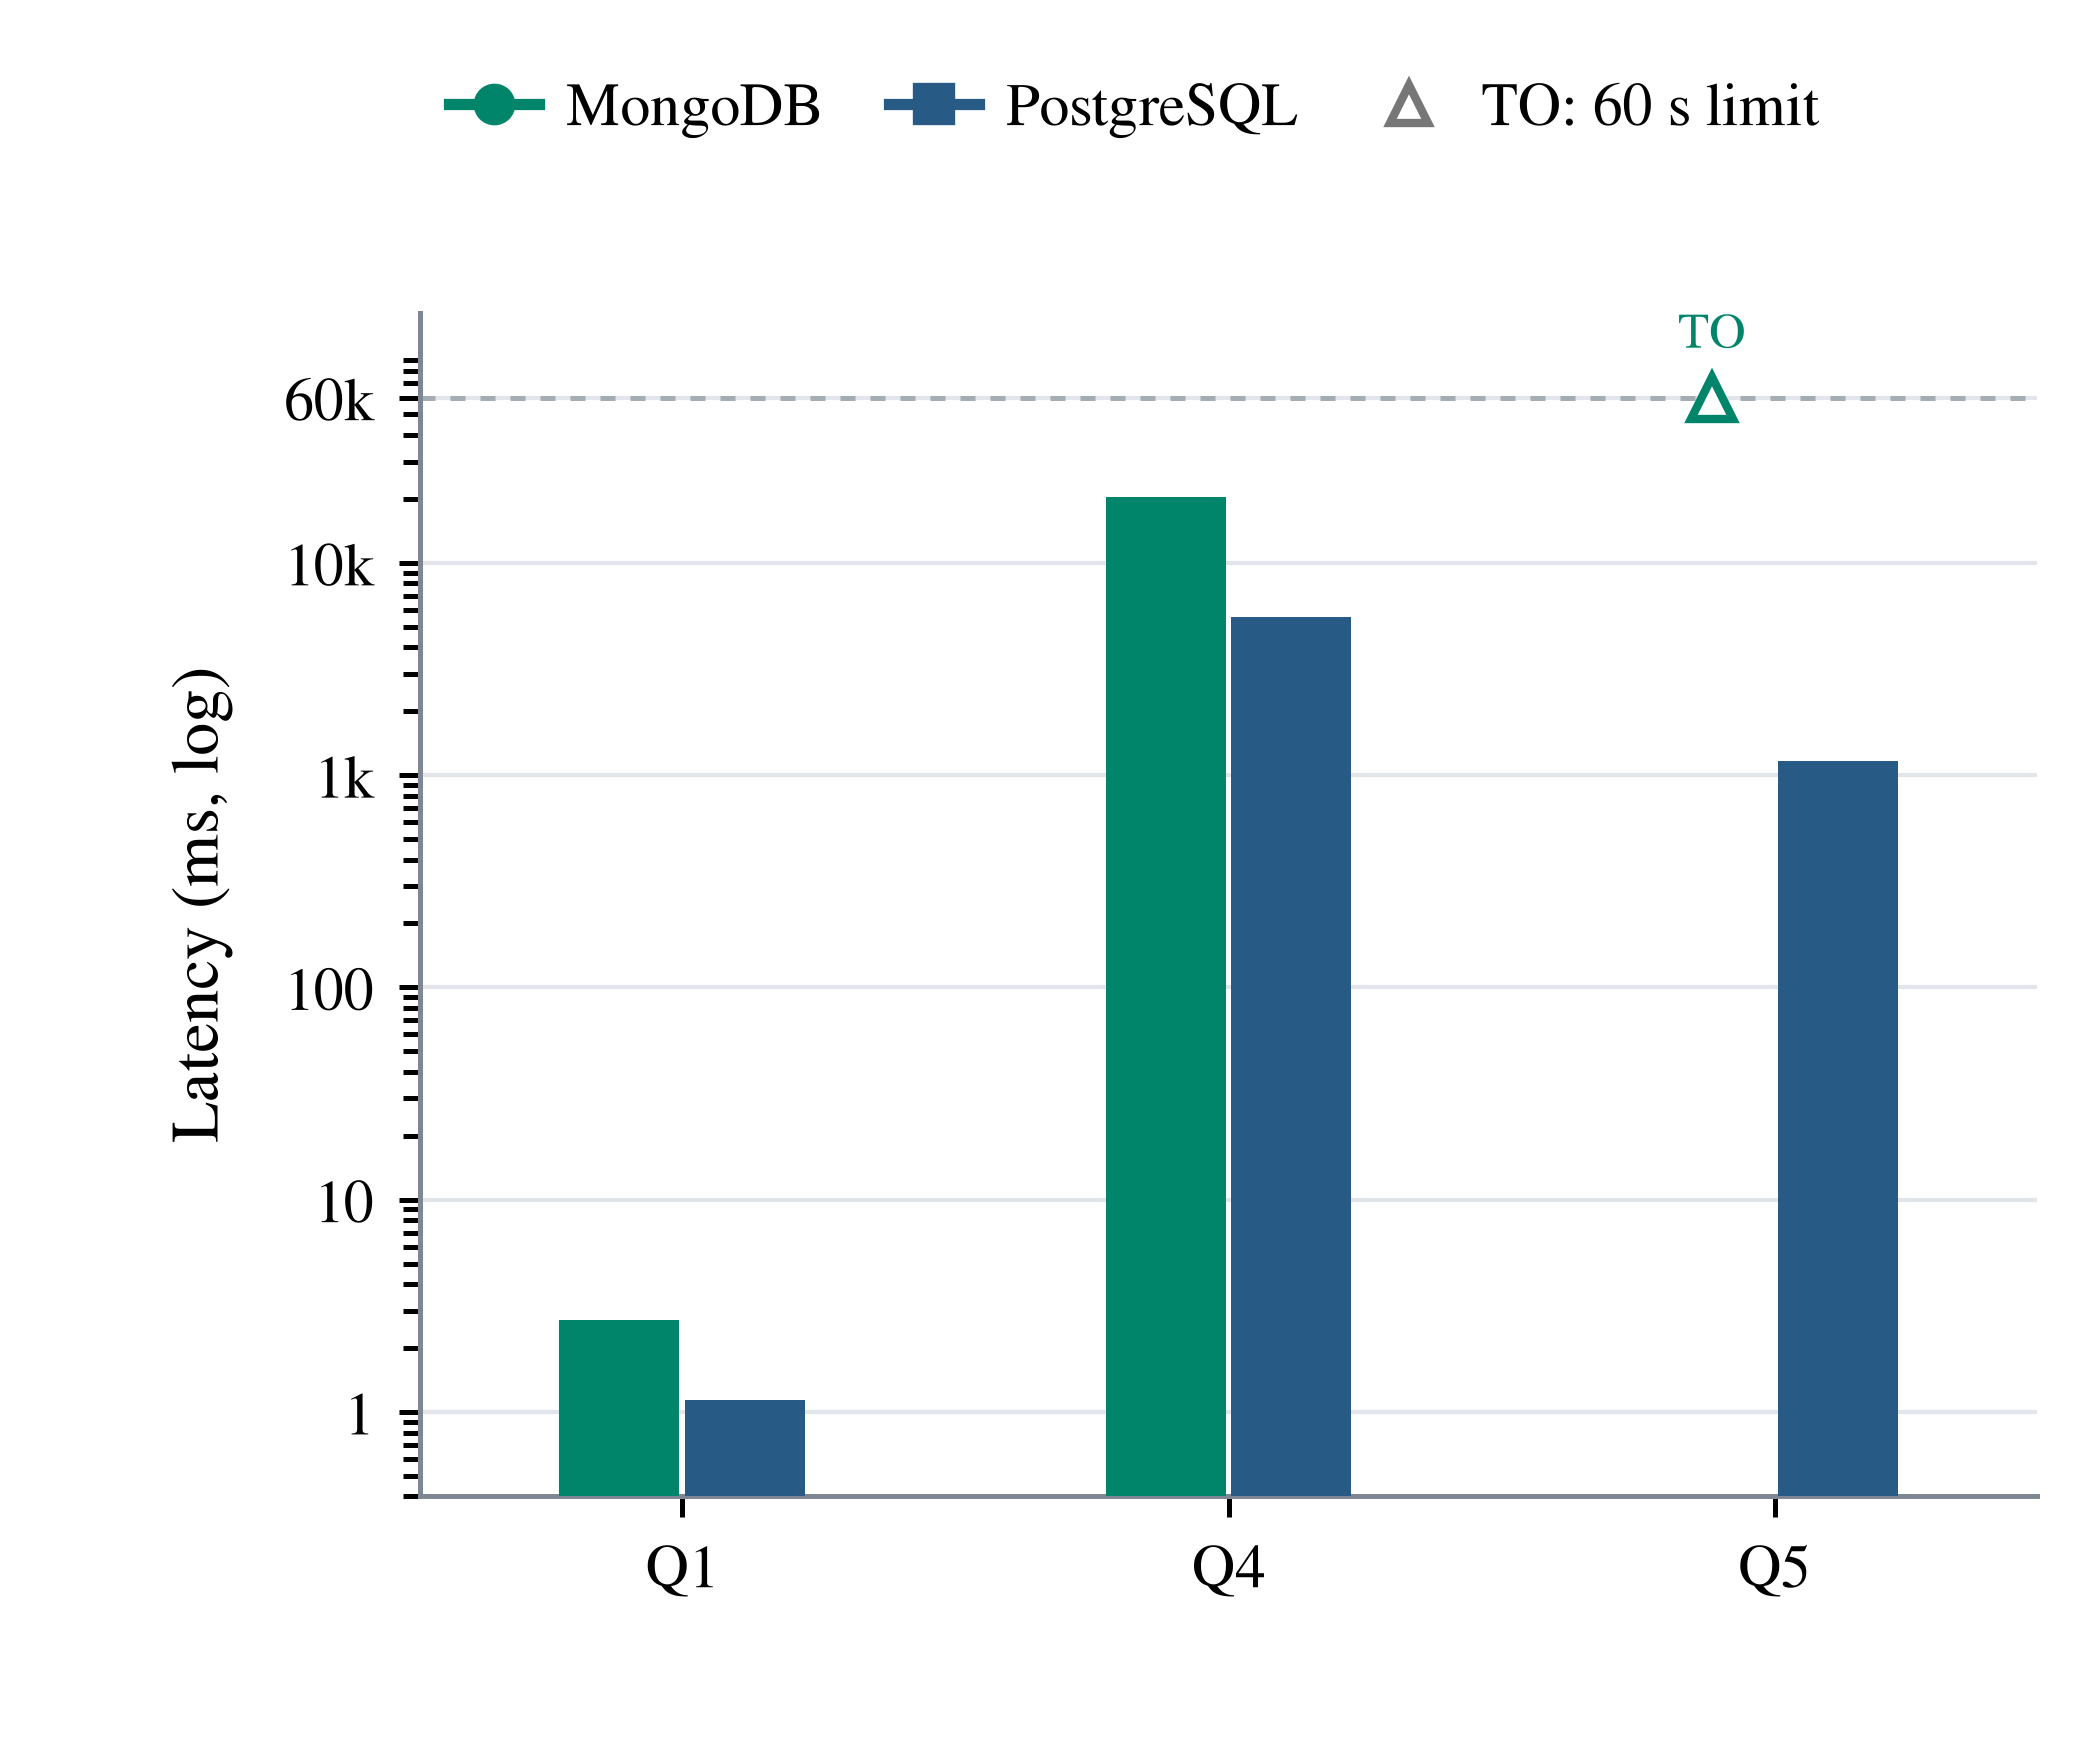
\includegraphics[width=\linewidth]{fig8_complexity_breakdown.png}
  \caption{Median indexed-query latency at SF~1.0 on a logarithmic axis. TO marks the 60-second server limit.}
  \label{fig:complexity}
\end{figure}

\begin{figure}[htbp]
  \centering
  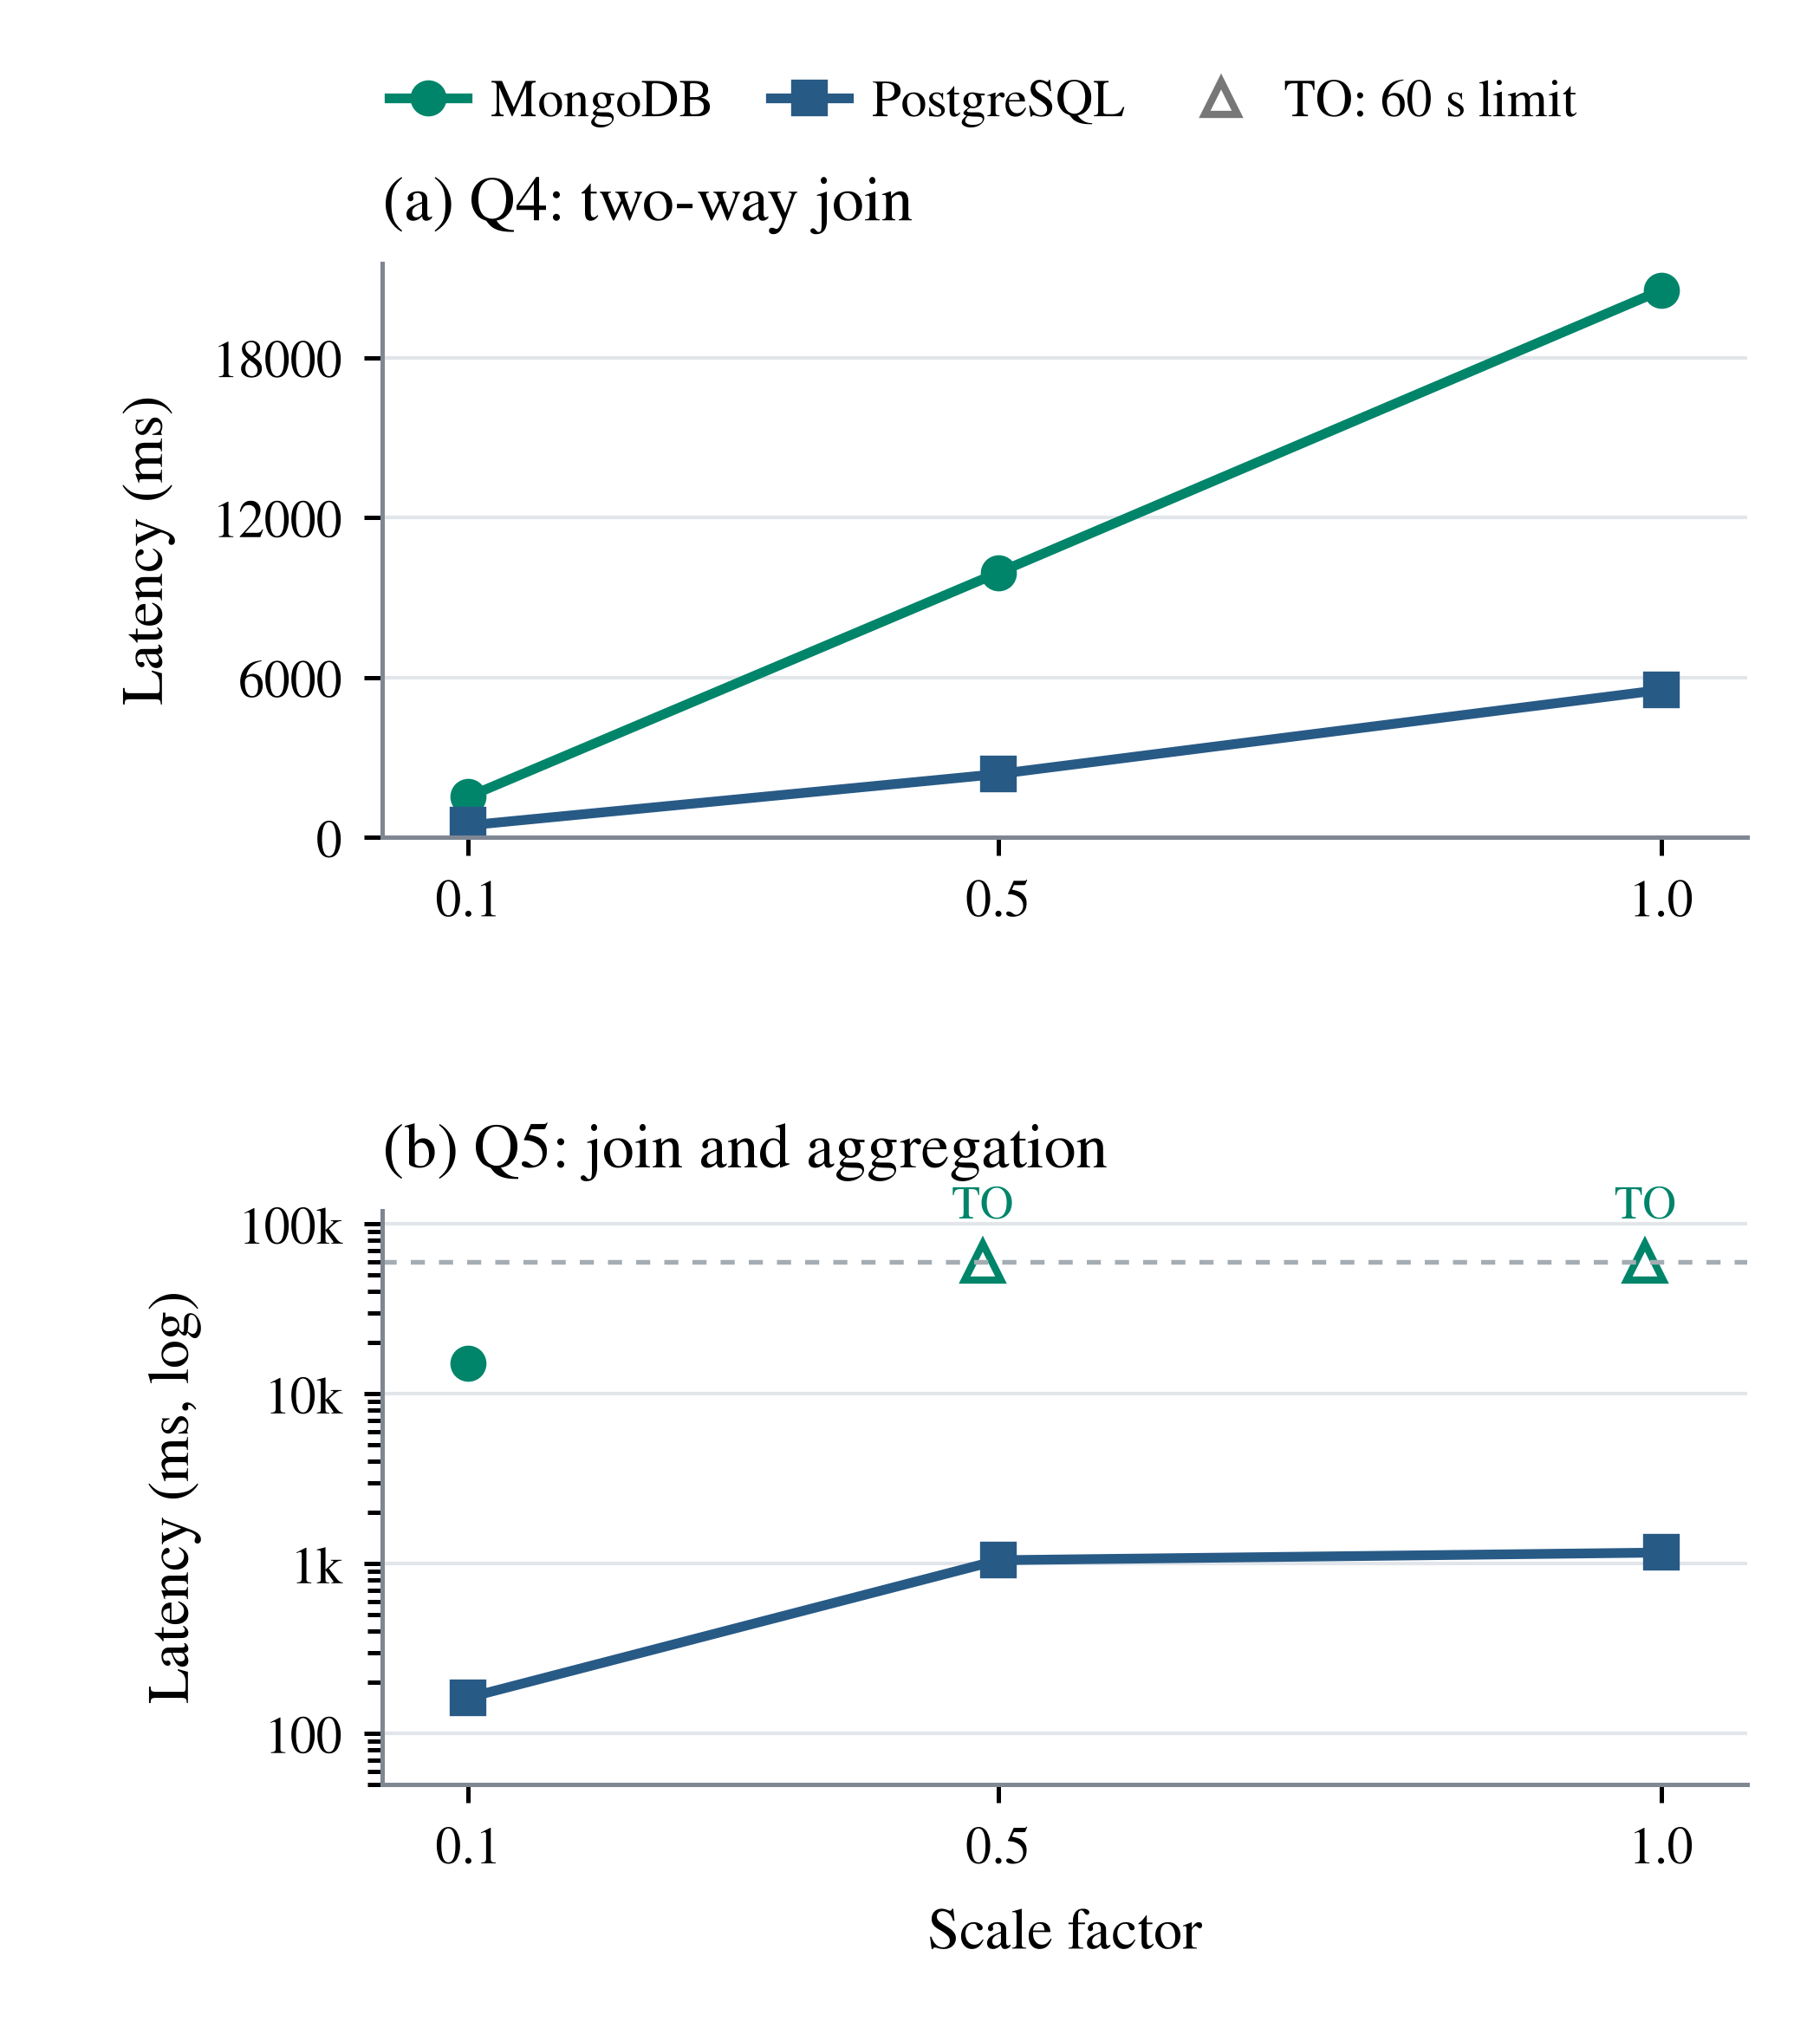
\includegraphics[width=\linewidth]{fig9_join_aggregation_deepdive.png}
  \caption{Median indexed join and aggregation latency across scale factors. TO marks the server limit; no median is inferred for a timeout.}
  \label{fig:joinagg}
\end{figure}

\subsection{Data Volume~$\times$~Query Complexity Interaction}
Table~\ref{tab:master} retains the planned $3\times6$ matrix. 10 core-query comparisons completed with matching outputs. 10 of the 10 complete core-query comparisons had Holm-adjusted $p<0.05$ across the full family of completed query comparisons. The ratio is $R=L_{\mathrm{MongoDB}}/L_{\mathrm{PostgreSQL}}$, computed from unrounded medians. The speedup divides the slower median by the faster one. Table $p$-values are unadjusted, two-sided Mann--Whitney results. Missing comparisons have no assigned winner or inferred $p$-value.

%% ── Table 3: Master Latency Matrix (spans both columns) ─────────────
\begin{table*}[t]
\caption{Master Latency \& Performance-Ratio Matrix
  ($R < 1$: MongoDB faster;\; $R > 1$: PostgreSQL faster)}
\label{tab:master}
\centering\small
\renewcommand{\arraystretch}{1.2}
\begin{adjustbox}{max width=\textwidth}
\begin{tabular}{@{}llllrrrrlc@{}}
\toprule
\textbf{Phase} & \textbf{SF} & \textbf{Workload} & \textbf{Index Mode}
  & \textbf{MongoDB (ms)} & \textbf{PostgreSQL (ms)}
  & \textbf{Ratio ($R$)} & \textbf{Speedup}
  & \textbf{Winner} & \textbf{$p$-value} \\ \midrule
Small & 0.1 & $Q1$ (Equality) & none & 8.34 & 0.61 & 13.72 & $13.72\times$ & \textbf{PostgreSQL} & 0.000183 \\
Small & 0.1 & $Q1$ (Equality) & indexed & 1.22 & 0.67 & 1.83 & $1.83\times$ & \textbf{PostgreSQL} & 0.00283 \\
Small & 0.1 & $Q4$ (Join) & none & \textit{TO} & 366.33 & -- & -- & -- & -- \\
Small & 0.1 & $Q4$ (Join) & indexed & 1530.13 & 459.48 & 3.33 & $3.33\times$ & \textbf{PostgreSQL} & 0.000183 \\
Small & 0.1 & $Q5$ (Aggregate) & none & \textit{TO} & 208.97 & -- & -- & -- & -- \\
Small & 0.1 & $Q5$ (Aggregate) & indexed & 15121.88 & 162.80 & 92.89 & $92.89\times$ & \textbf{PostgreSQL} & 0.000183 \\
Medium & 0.5 & $Q1$ (Equality) & none & 36.99 & 0.55 & 67.60 & $67.60\times$ & \textbf{PostgreSQL} & 0.000183 \\
Medium & 0.5 & $Q1$ (Equality) & indexed & 2.79 & 1.18 & 2.35 & $2.35\times$ & \textbf{PostgreSQL} & 0.000183 \\
Medium & 0.5 & $Q4$ (Join) & none & \textit{TO} & 2126.19 & -- & -- & -- & -- \\
Medium & 0.5 & $Q4$ (Join) & indexed & 9937.65 & 2384.42 & 4.17 & $4.17\times$ & \textbf{PostgreSQL} & 0.000183 \\
Medium & 0.5 & $Q5$ (Aggregate) & none & \textit{TO} & 925.41 & -- & -- & -- & -- \\
Medium & 0.5 & $Q5$ (Aggregate) & indexed & \textit{TO} & 1049.07 & -- & -- & -- & -- \\
Large & 1.0 & $Q1$ (Equality) & none & 270.22 & 1.16 & 232.46 & $232.46\times$ & \textbf{PostgreSQL} & 0.000183 \\
Large & 1.0 & $Q1$ (Equality) & indexed & 2.71 & 1.14 & 2.38 & $2.38\times$ & \textbf{PostgreSQL} & 0.000246 \\
Large & 1.0 & $Q4$ (Join) & none & \textit{TO} & \textit{TO} & -- & -- & -- & -- \\
Large & 1.0 & $Q4$ (Join) & indexed & 20521.51 & 5538.78 & 3.71 & $3.71\times$ & \textbf{PostgreSQL} & 0.000183 \\
Large & 1.0 & $Q5$ (Aggregate) & none & \textit{TO} & 1672.61 & -- & -- & -- & -- \\
Large & 1.0 & $Q5$ (Aggregate) & indexed & \textit{TO} & 1163.76 & -- & -- & -- & -- \\
\bottomrule
\end{tabular}
\end{adjustbox}
\end{table*}
%%─────────────────────────────────────────────────────────────────────

\subsection{CRUD Performance}
Figure~\ref{fig:insert} and Figure~\ref{fig:crud} report measured insert throughput and CRUD batch latency. The row counts are checked for every trial. Variability is summarized from actual repetitions, and no causal attribution to background storage-engine activity is made. For indexed SF~1.0, the 50-record key-read batch had median latency of 43.51\,ms for MongoDB and 20.64\,ms for PostgreSQL. The corresponding throughputs were 1{,}149 and 2{,}423 records/s, with a reported $2.11\times$ PostgreSQL speedup.

\subsection{Indexing Impact}
Figure~\ref{fig:index} compares measured read medians with and without the optional workload indexes. The change is calculated separately for each completed engine/workload configuration. Across complete pairs of index configurations, the observed unindexed-to-indexed median ratio ranged from 0.46 to 1583.76. A ratio above 1 indicates a lower indexed median, and a ratio below 1 indicates a higher indexed median. Table~\ref{tab:plans} and Figure~\ref{fig:plandiag} report executed-plan diagnostics. For the baseline equality lookup, PostgreSQL retains a business-key primary-key access path while MongoDB scans for a business key distinct from its mandatory identifier. This is an access-path difference within the tested schema, so it cannot establish an inherent point-lookup advantage for either storage model. Planning time is distinct from execution time. Shared-buffer hits count buffer accesses, rather than distinct disk blocks. Incomplete plans are marked NM.

\begin{figure}[htbp]
  \centering
  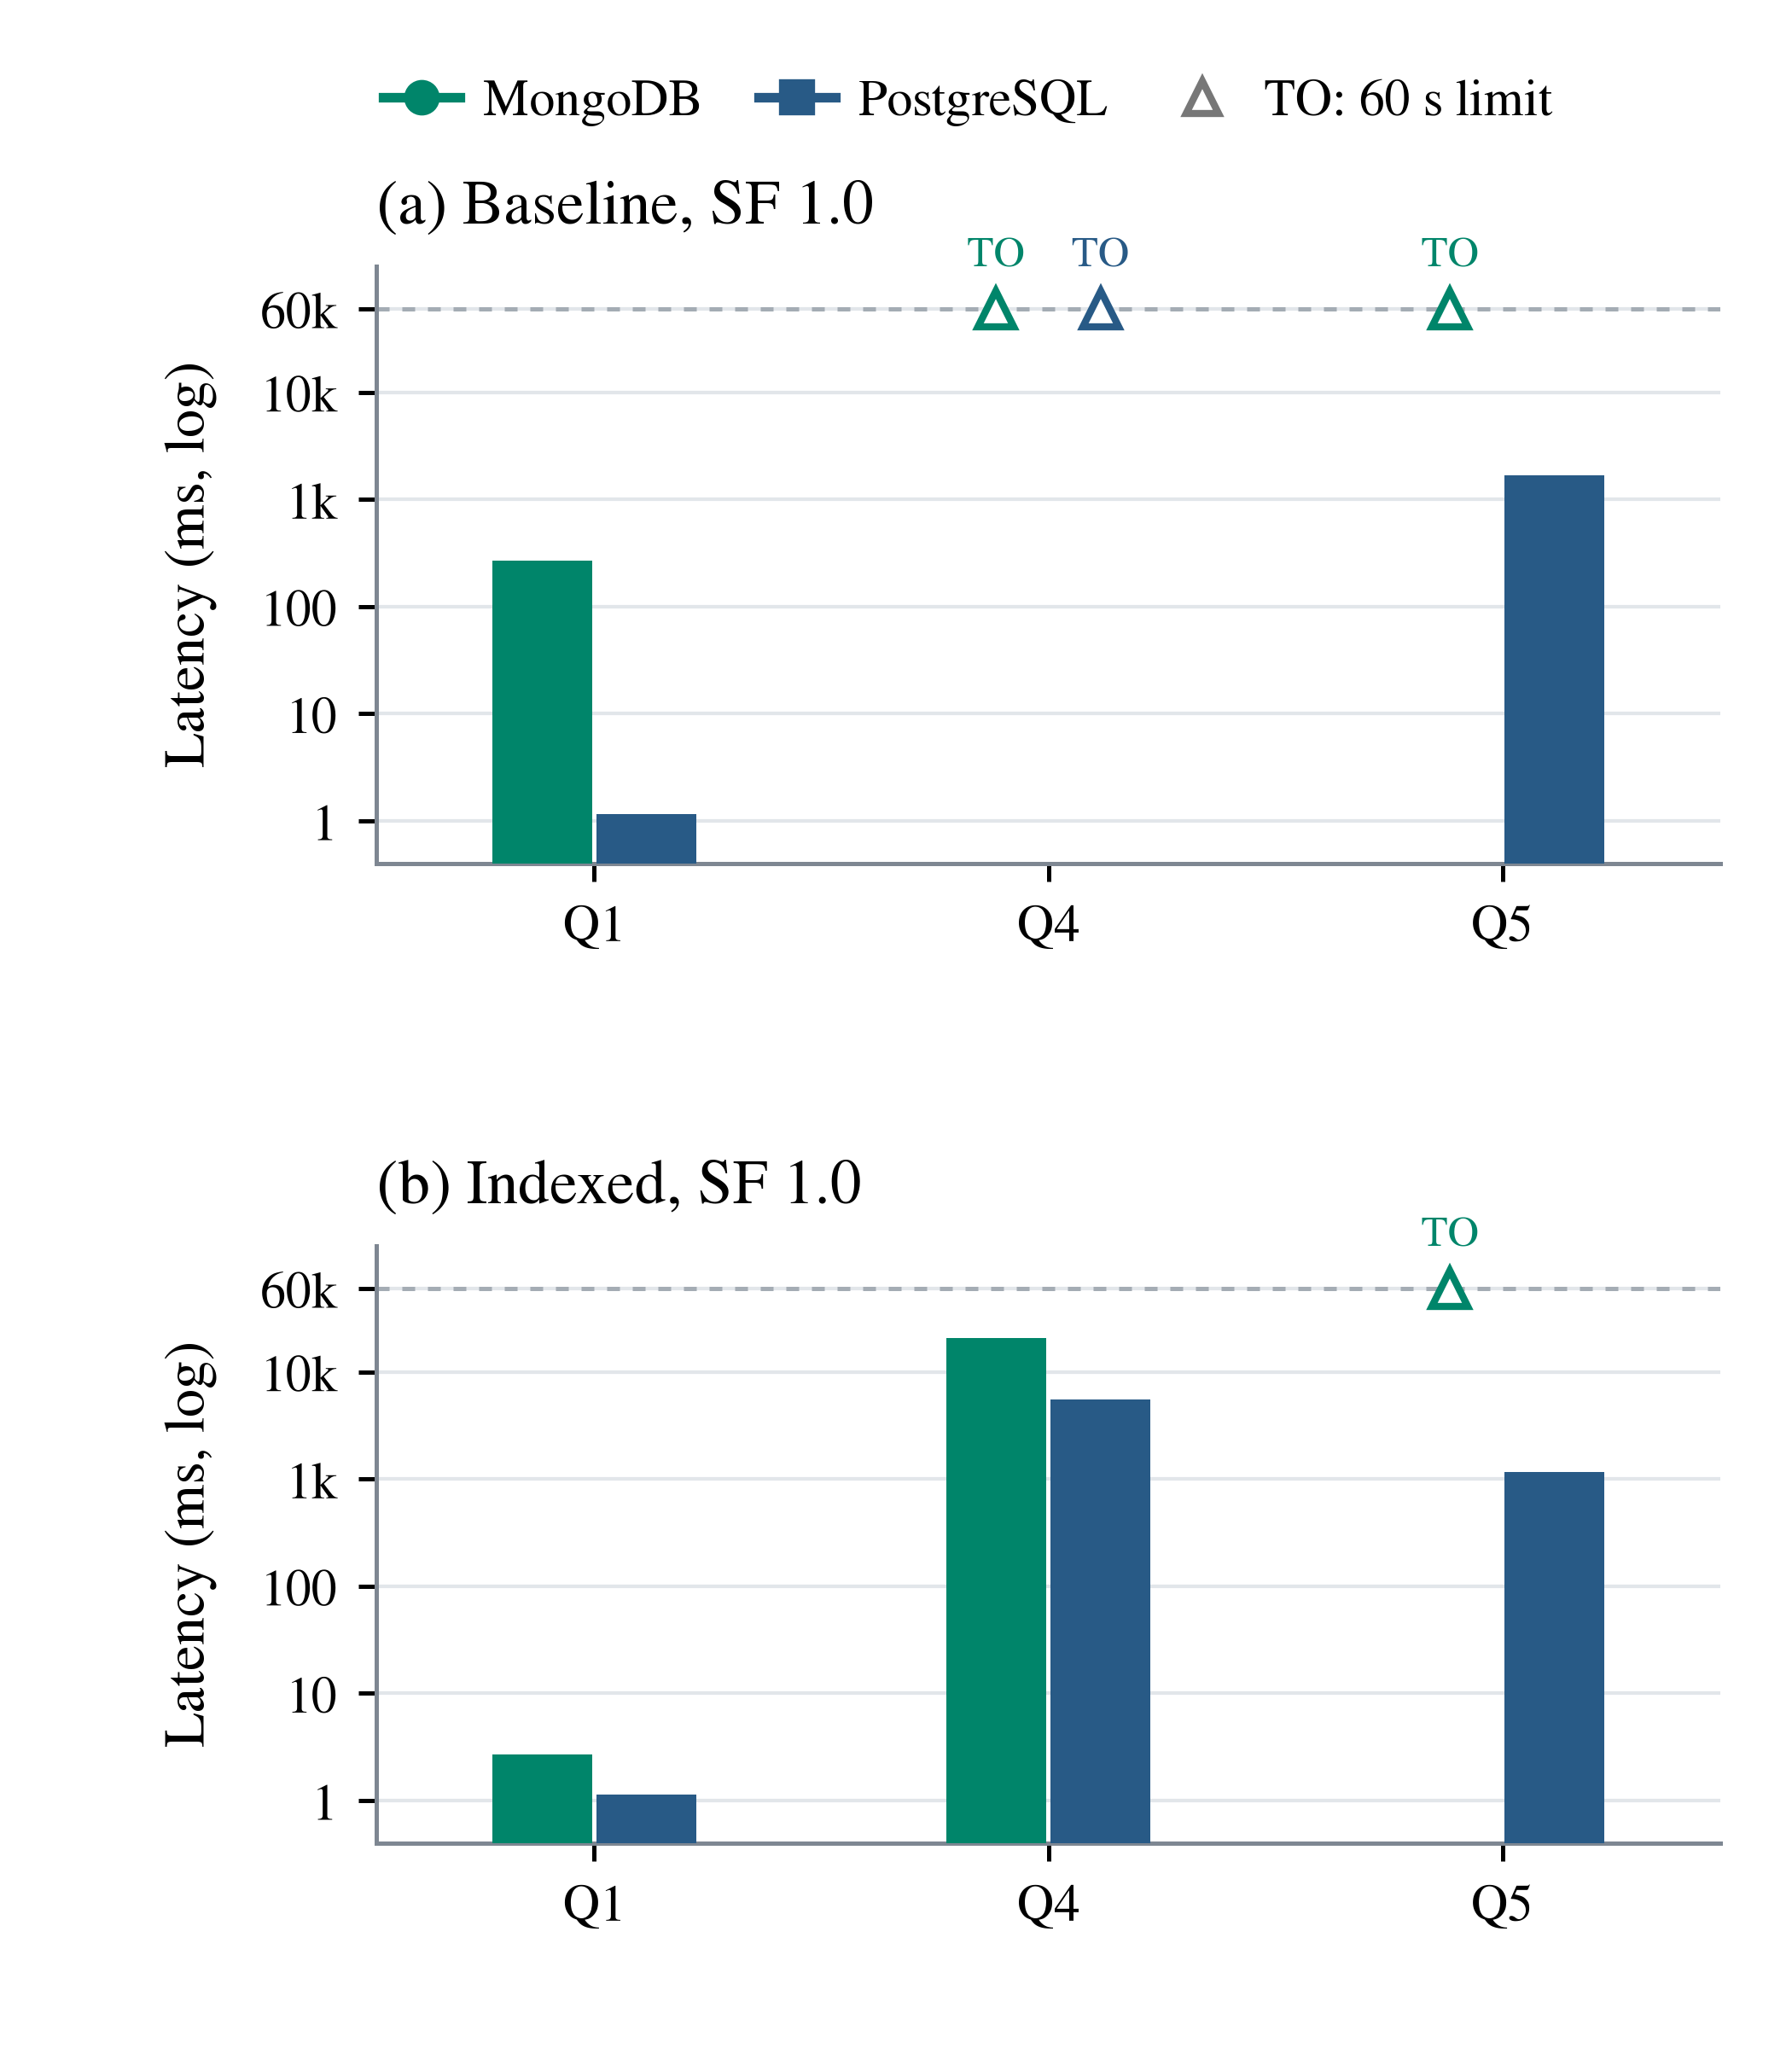
\includegraphics[width=\linewidth]{fig10_index_impact.png}
  \caption{Median latency with and without optional indexes at SF~1.0, using identical logarithmic axes. TO marks the server limit.}
  \label{fig:index}
\end{figure}

%% ── Table 4: Execution-Plan Diagnostics (spans both columns) ─────────
\begin{table*}[t]
\caption{Query Execution-Plan Diagnostics: Physical Scan Types and Memory Block Counts}
\label{tab:plans}
\centering\small
\renewcommand{\arraystretch}{1.2}
\setlength{\tabcolsep}{5pt}
\begin{adjustbox}{max width=\textwidth}
\begin{tabular}{@{}cclcrrcrr@{}}
\toprule
\textbf{SF} & \textbf{Workload} & \textbf{Index Mode}
  & \multicolumn{3}{c}{\textbf{MongoDB}}
  & \multicolumn{3}{c}{\textbf{PostgreSQL}} \\
\cmidrule(lr){4-6}\cmidrule(lr){7-9}
 & & & \textbf{Stage} & \textbf{Docs Examined} & \textbf{Keys Examined}
   & \textbf{Plan Node} & \textbf{Plan Time} & \textbf{Shared Hit} \\ \midrule
0.1 & $Q1$ & none & PROJECTION\_SIMPLE / COLLSCAN & 15000 & 0 & Index Scan & 0.079 & 3 \\
0.1 & $Q1$ & indexed & PROJECTION\_SIMPLE / FETCH / IXSCAN & 1 & 1 & Index Scan & 0.157 & 3 \\
0.1 & $Q4$ & none & NM & NM & NM & Hash Join & 0.191 & 2316 \\
0.1 & $Q4$ & indexed & PROJECTION\_SIMPLE / FETCH / IXSCAN & 32967 & 32967 & Hash Join & 0.418 & 2238 \\
0.5 & $Q1$ & none & PROJECTION\_SIMPLE / COLLSCAN & 75000 & 0 & Index Scan & 0.122 & 3 \\
0.5 & $Q1$ & indexed & PROJECTION\_SIMPLE / FETCH / IXSCAN & 1 & 1 & Index Scan & 0.195 & 0 \\
1.0 & $Q1$ & none & PROJECTION\_SIMPLE / COLLSCAN & 150000 & 0 & Index Scan & 0.163 & 4 \\
1.0 & $Q1$ & indexed & PROJECTION\_SIMPLE / FETCH / IXSCAN & 1 & 1 & Index Scan & 0.091 & 0 \\
1.0 & $Q5$ & indexed & NM & NM & NM & Sort & 0.369 & 13126 \\
\bottomrule
\end{tabular}
\end{adjustbox}
\end{table*}
%%─────────────────────────────────────────────────────────────────────

\begin{figure}[htbp]
  \centering
  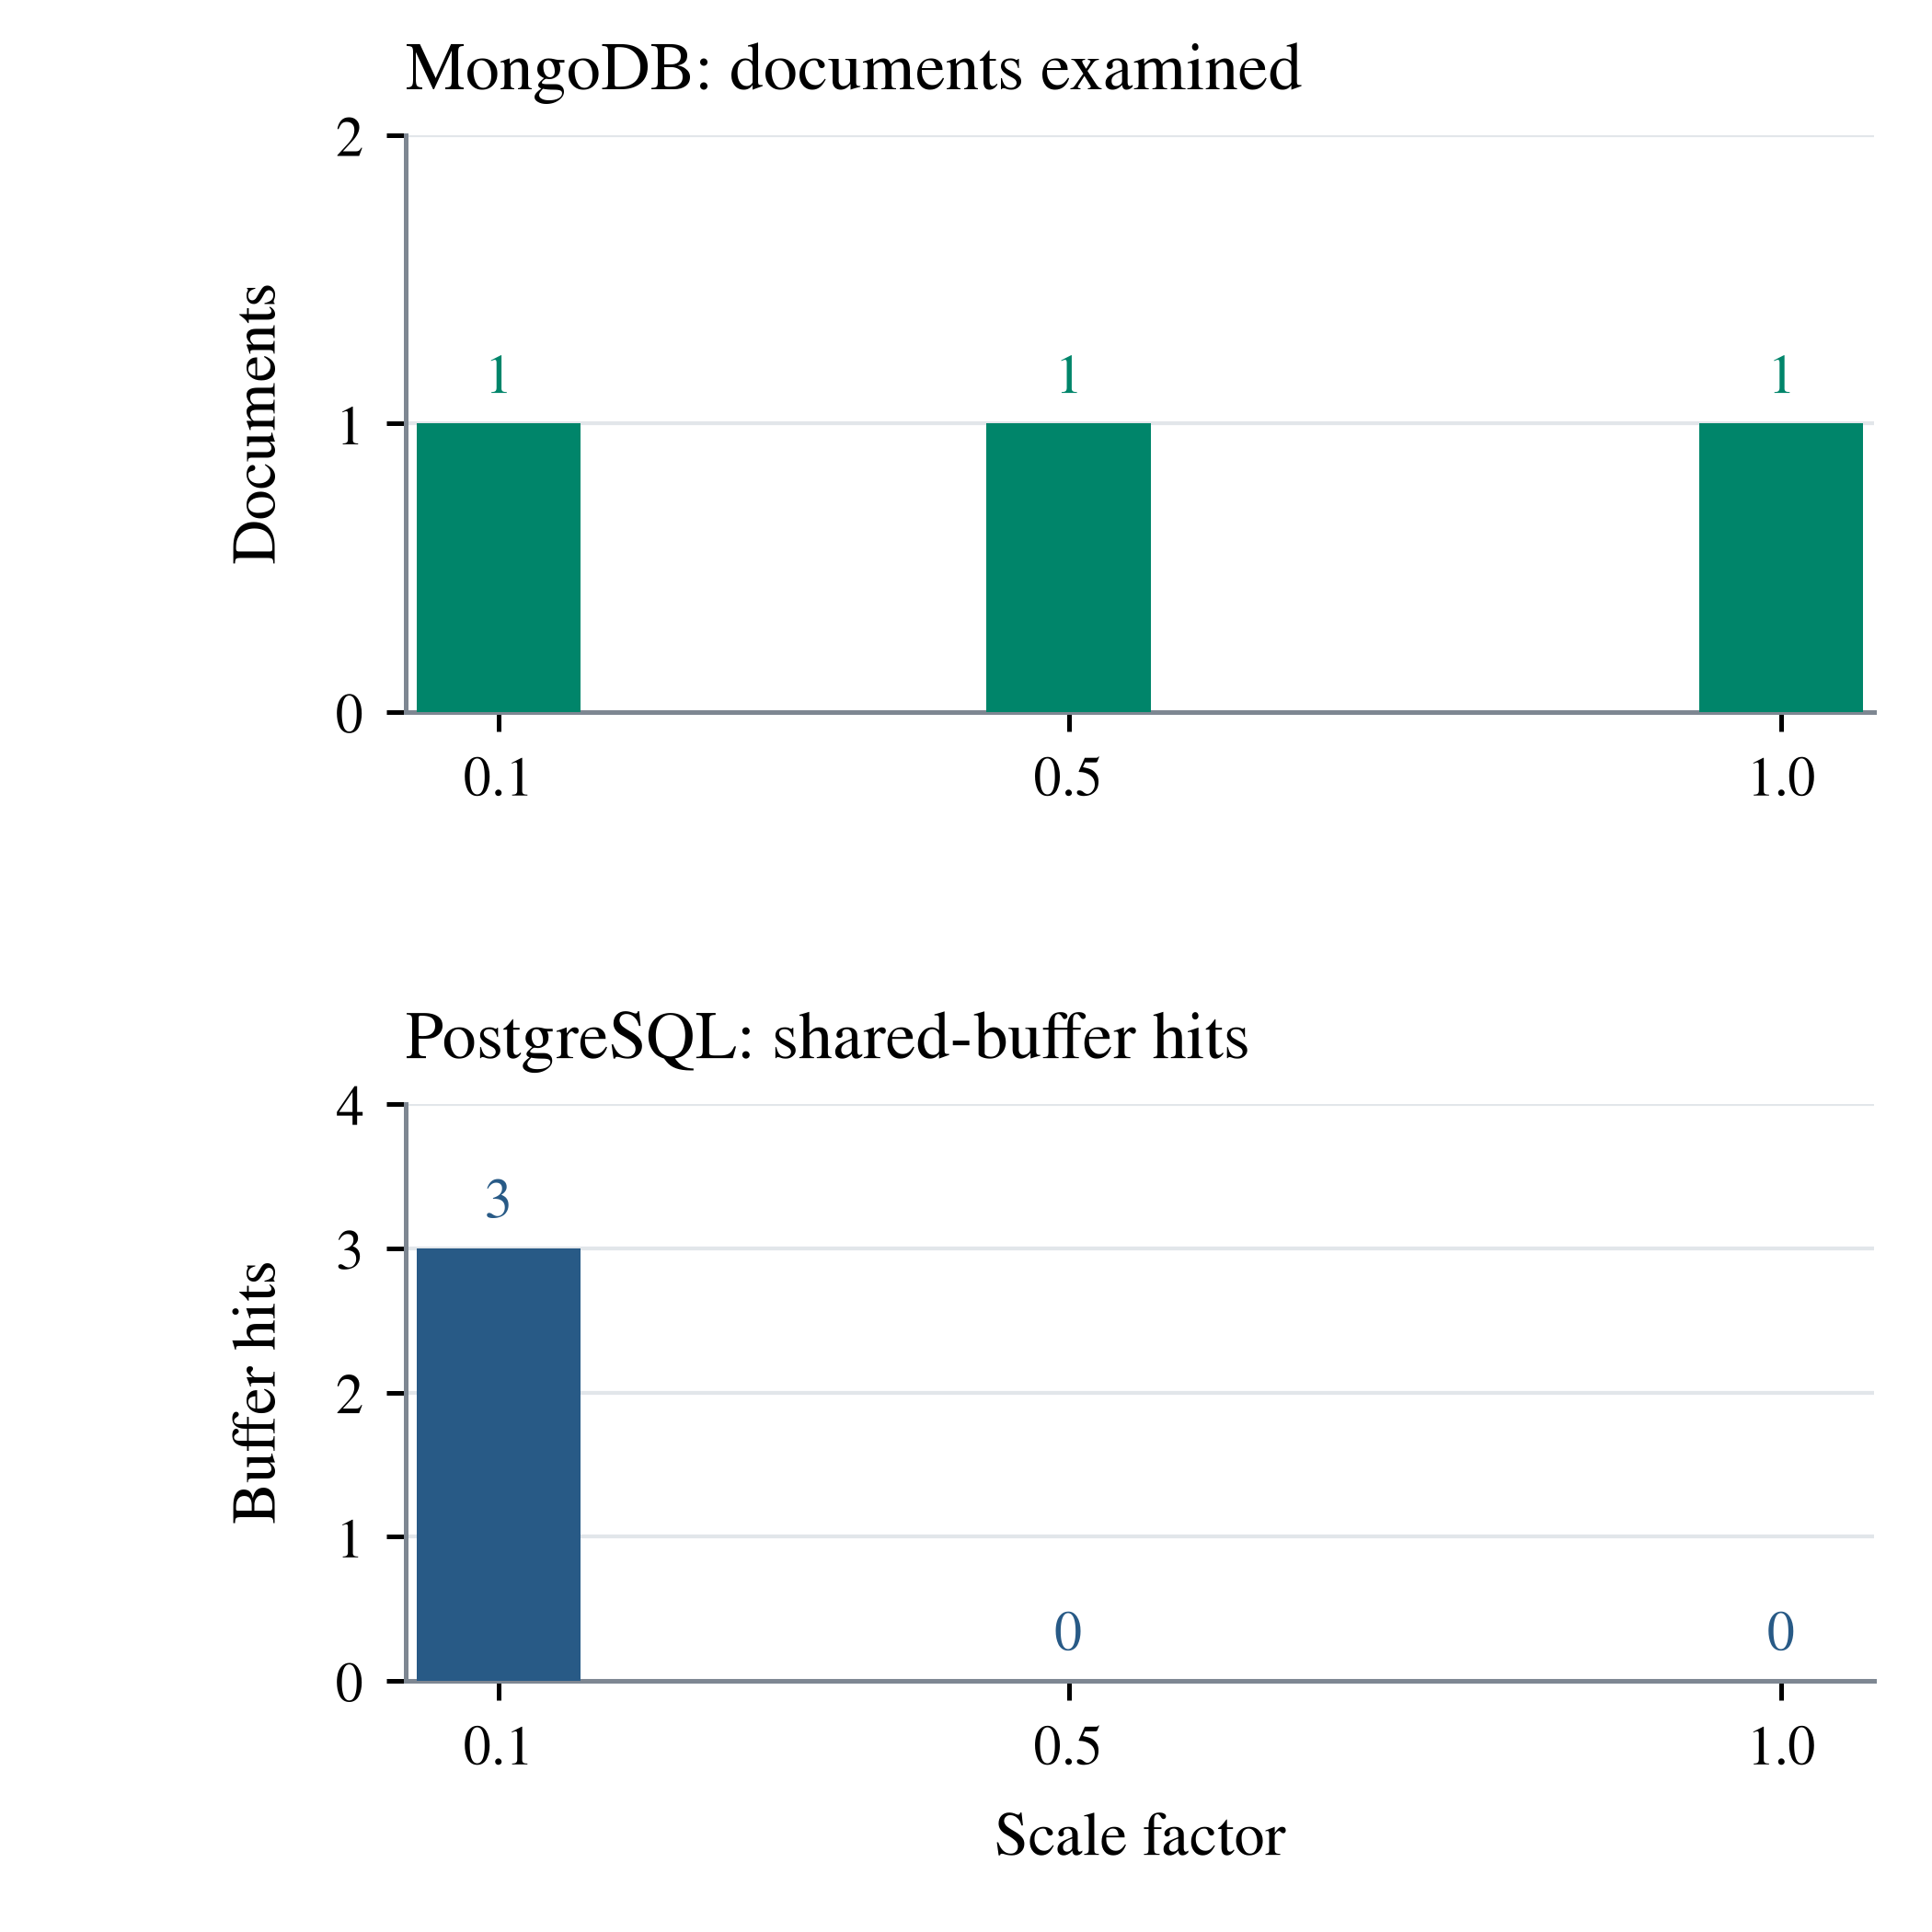
\includegraphics[width=\linewidth]{fig13_execution_plan_diagnostics.png}
  \caption{Indexed $Q1$ execution-plan counters. MongoDB documents examined and PostgreSQL shared-buffer hits have different meanings. Zero shared hits are reported as recorded.}
  \label{fig:plandiag}
\end{figure}

\subsection{Storage Analysis}
Table~\ref{tab:storage} and Figure~\ref{fig:storage} use measured allocated data and index bytes. Raw size is the sum of the eight CSV file sizes. All displayed sizes use MiB ($2^{20}$ bytes). PostgreSQL data allocation includes table and auxiliary storage, with indexes reported separately. MongoDB data allocation uses \texttt{storageSize}, and its indexes use \texttt{indexSize}. Uncompressed BSON \texttt{dataSize} is retained separately in the evidence. The storage ratio uses allocated data plus indexes divided by raw CSV bytes. At SF~1.0 with optional indexes, the measured allocated-storage ratios were $1.00\times$ for MongoDB and $1.68\times$ for PostgreSQL. PostgreSQL WAL and MongoDB journal files are excluded from this table/collection-and-index comparison. Both servers were explicitly checkpointed before the storage snapshots.

%% ── Table 5: Storage Footprint (spans both columns) ──────────────────
\begin{table*}[t]
\caption{Storage footprint and index overhead (MiB), relative to raw CSV size}
\label{tab:storage}
\centering\small
\renewcommand{\arraystretch}{1.2}
\begin{adjustbox}{max width=\textwidth}
\begin{tabular}{@{}llrlrrrrrrrr@{}}
\toprule
\textbf{Phase} & \textbf{SF} & \textbf{Raw CSV} & \textbf{Index Mode}
  & \multicolumn{4}{c}{\textbf{MongoDB}}
  & \multicolumn{4}{c}{\textbf{PostgreSQL}} \\
\cmidrule(lr){5-8}\cmidrule(lr){9-12}
 & & & & \textbf{Data} & \textbf{Index} & \textbf{Total} & \textbf{Ratio}
   & \textbf{Data} & \textbf{Index} & \textbf{Total} & \textbf{Ratio} \\ \midrule
Small & 0.1 & 87.91 & none & 68.43 & 8.72 & 77.15 & $0.88\times$ & 113.12 & 26.69 & 139.80 & $1.59\times$ \\
Small & 0.1 & 87.91 & indexed & 68.43 & 24.71 & 93.14 & $1.06\times$ & 113.12 & 48.52 & 161.63 & $1.84\times$ \\
Medium & 0.5 & 449.36 & none & 342.42 & 44.86 & 387.27 & $0.86\times$ & 563.50 & 92.98 & 656.48 & $1.46\times$ \\
Medium & 0.5 & 449.36 & indexed & 342.42 & 118.61 & 461.02 & $1.03\times$ & 563.50 & 201.55 & 765.05 & $1.70\times$ \\
Large & 1.0 & 909.85 & none & 685.13 & 91.44 & 776.57 & $0.85\times$ & 1126.45 & 185.73 & 1312.18 & $1.44\times$ \\
Large & 1.0 & 909.85 & indexed & 685.13 & 225.13 & 910.26 & $1.00\times$ & 1126.45 & 402.11 & 1528.55 & $1.68\times$ \\
\bottomrule
\end{tabular}
\end{adjustbox}
\end{table*}
%%─────────────────────────────────────────────────────────────────────

\begin{figure}[htbp]
  \centering
  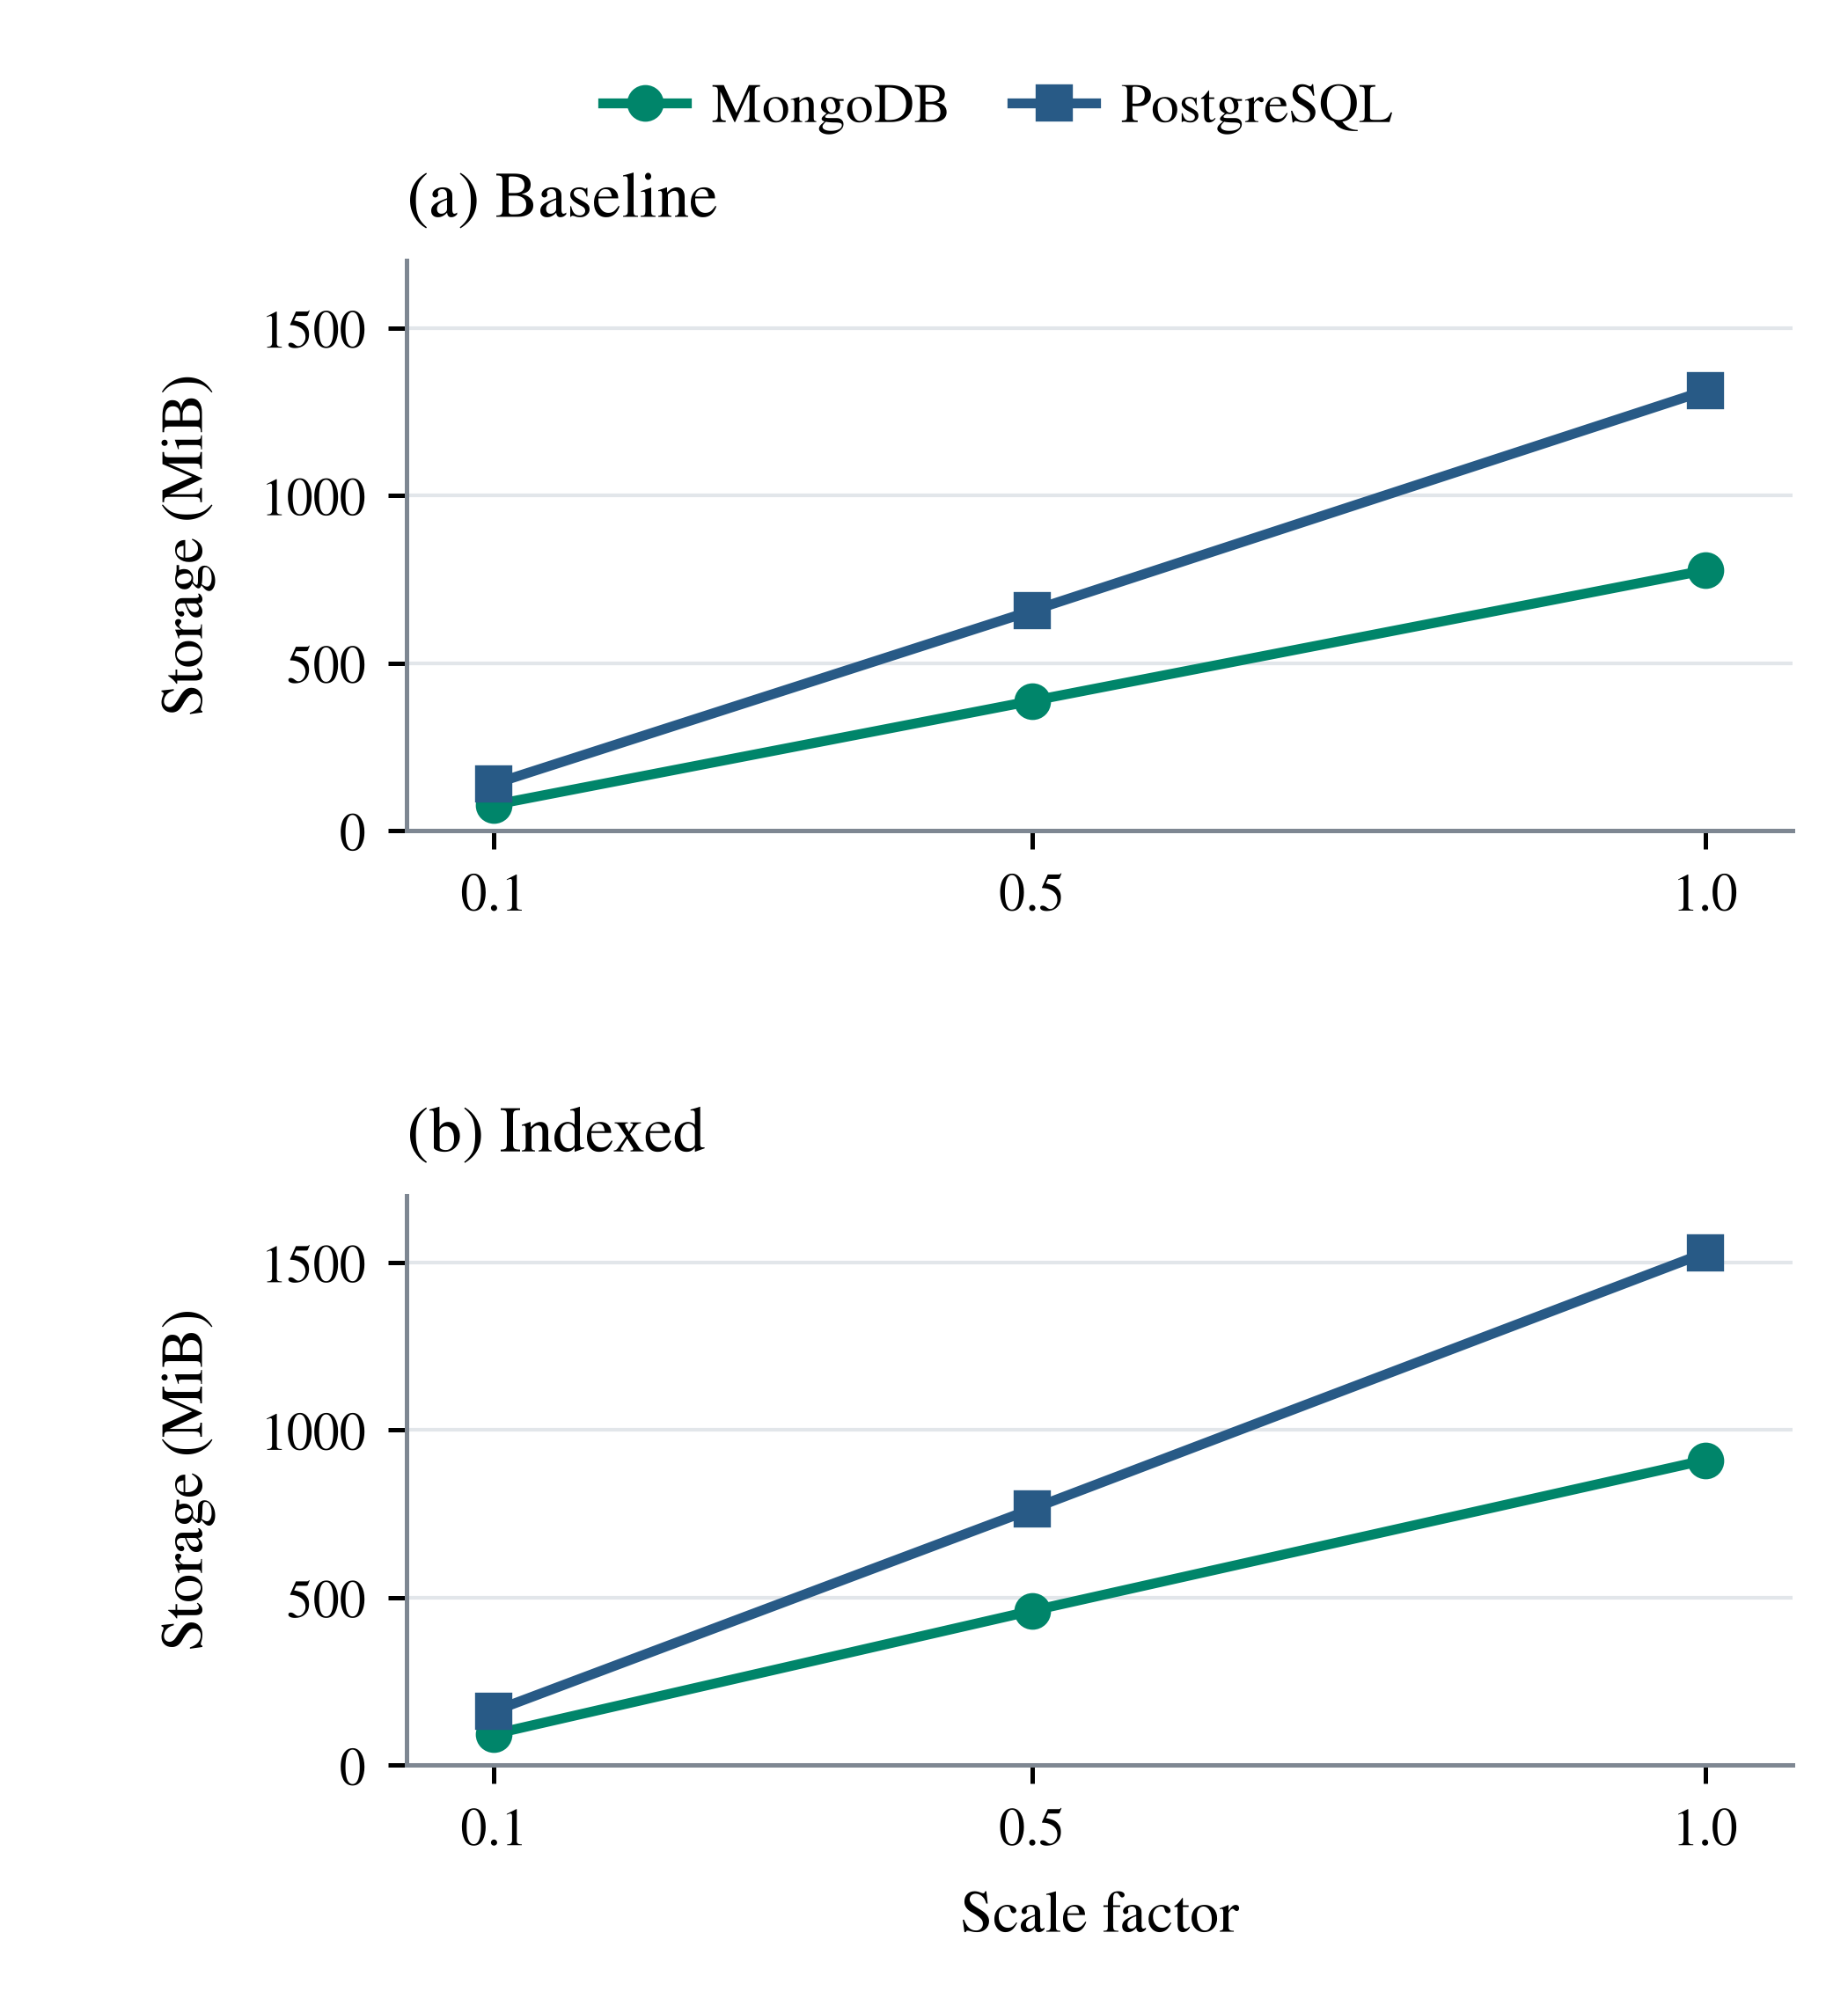
\includegraphics[width=\linewidth]{fig11_storage_analysis.png}
  \caption{Measured allocated data plus index storage. Ratios use the corresponding exported or generated CSV byte totals.}
  \label{fig:storage}
\end{figure}

\subsection{Scalability and Resource Utilization}
Table~\ref{tab:resources} and Figure~\ref{fig:resource} report sampled local server-process CPU and aggregate RSS. CPU sums per-process rates and normalizes by the 24 logical processors. Process RSS is sampled at 50-ms intervals and at query boundaries, with the arithmetic mean reported across runs. PostgreSQL includes the running instance\textquotesingle s processes and other backends. Summed RSS may count shared pages more than once, and parallel workers created after enumeration may be missed. Short-query CPU rates are limited by operating-system accounting resolution. These measurements describe observed process footprints and do not establish an equivalent reduction in physical RAM requirements.

%% ── Table 6: System Resource Utilization (spans both columns) ────────
\begin{table*}[t]
\caption{Sampled local server CPU (host-normalized) and summed process RSS (MiB)}
\label{tab:resources}
\centering\small
\renewcommand{\arraystretch}{1.2}
\begin{adjustbox}{max width=\textwidth}
\begin{tabular}{@{}llclrrrrrr@{}}
\toprule
\textbf{Phase} & \textbf{SF} & \textbf{Workload} & \textbf{Index Mode}
  & \multicolumn{3}{c}{\textbf{MongoDB}}
  & \multicolumn{3}{c}{\textbf{PostgreSQL}} \\
\cmidrule(lr){5-7}\cmidrule(lr){8-10}
 & & & & \textbf{Avg CPU} & \textbf{Peak CPU} & \textbf{RAM (RSS)}
   & \textbf{Avg CPU} & \textbf{Peak CPU} & \textbf{RAM (RSS)} \\ \midrule
Small & 0.1 & $Q1$ & none & 1.45\% & 7.71\% & 481.21 & 0.00\% & 0.00\% & 871.07 \\
Small & 0.1 & $Q4$ & indexed & 3.69\% & 6.14\% & 486.45 & 0.17\% & 0.46\% & 897.25 \\
Small & 0.1 & $Q5$ & indexed & 4.07\% & 6.89\% & 497.22 & 1.05\% & 2.98\% & 929.70 \\
Medium & 0.5 & $Q1$ & none & 3.75\% & 5.33\% & 1133.18 & 0.00\% & 0.00\% & 938.32 \\
Medium & 0.5 & $Q4$ & indexed & 3.72\% & 6.78\% & 1146.80 & 0.89\% & 3.92\% & 956.90 \\
Medium & 0.5 & $Q5$ & indexed & \textit{NM} & \textit{NM} & \textit{NM} & 4.73\% & 11.71\% & 964.16 \\
Large & 1.0 & $Q1$ & none & 3.97\% & 14.82\% & 1046.07 & 0.01\% & 0.13\% & 959.75 \\
Large & 1.0 & $Q4$ & indexed & 3.59\% & 7.58\% & 1057.78 & 1.66\% & 5.40\% & 934.61 \\
Large & 1.0 & $Q5$ & indexed & \textit{NM} & \textit{NM} & \textit{NM} & 6.19\% & 16.28\% & 954.94 \\
\bottomrule
\end{tabular}
\end{adjustbox}
\end{table*}
%%─────────────────────────────────────────────────────────────────────

\begin{figure}[htbp]
  \centering
  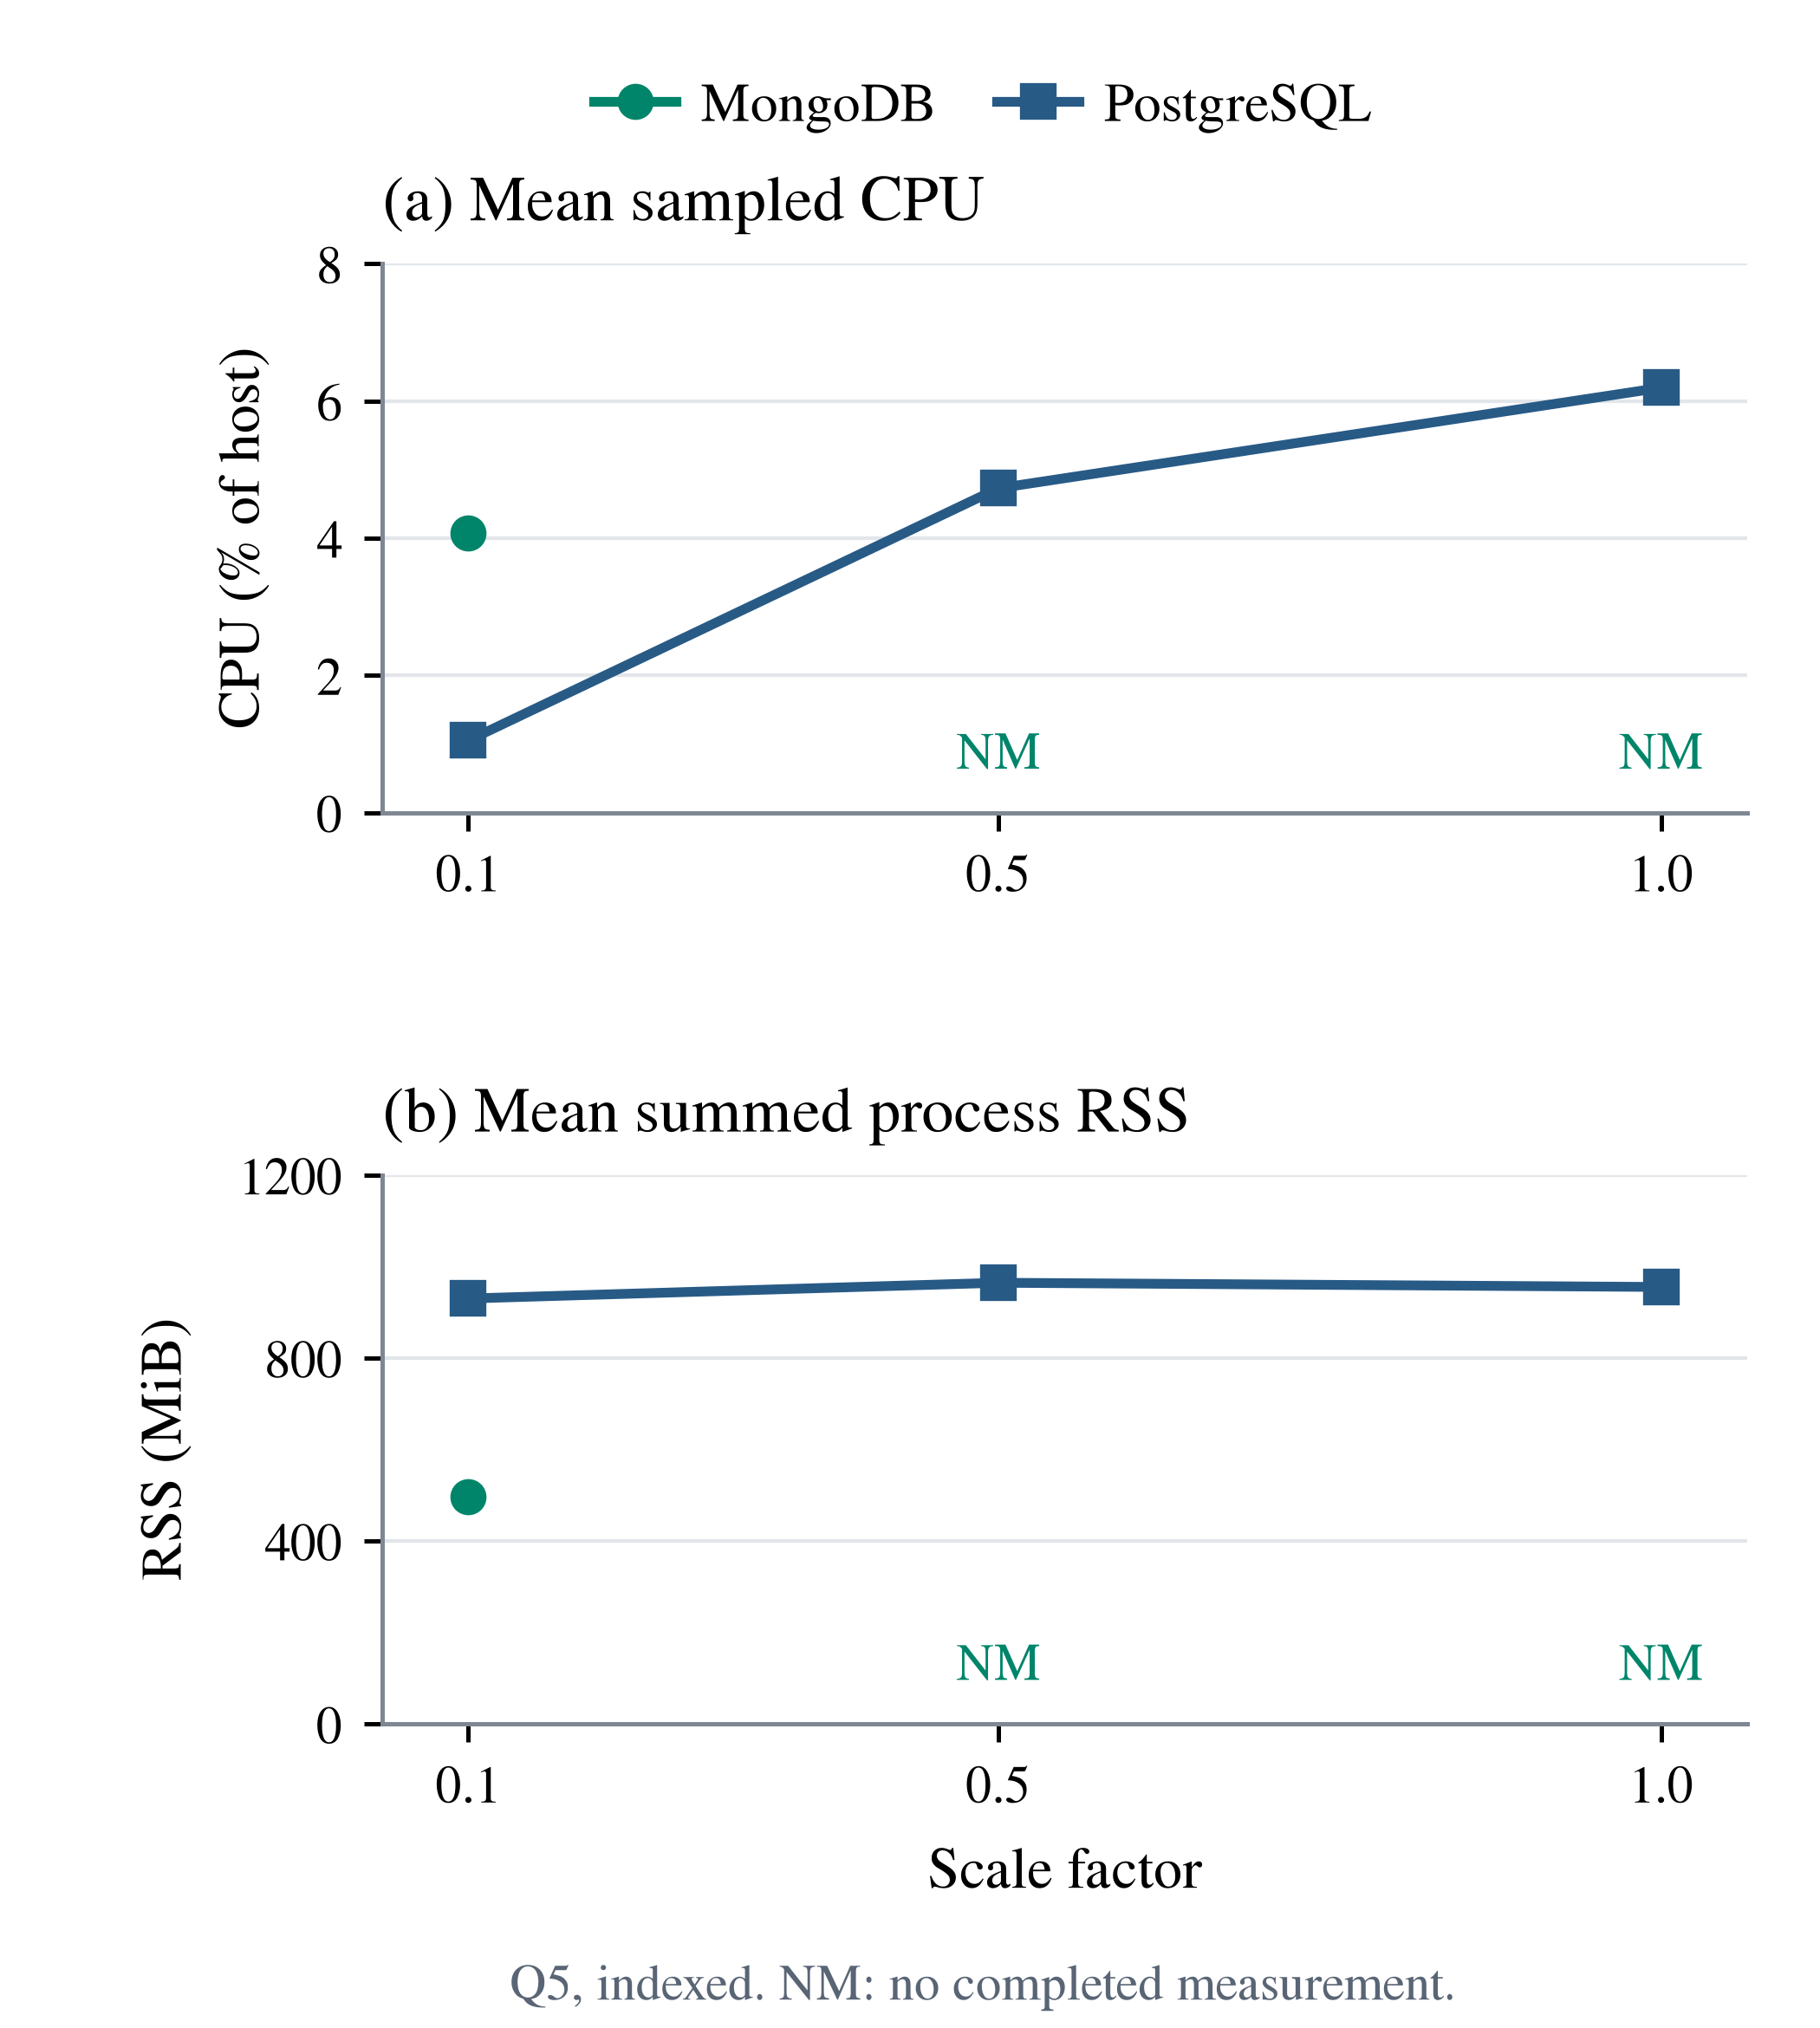
\includegraphics[width=\linewidth]{fig12_resource_utilization.png}
  \caption{Sampled CPU and summed process RSS for indexed $Q5$. NM denotes an unavailable complete measurement. RSS can double-count shared pages, and short-query CPU rates have limited resolution.}
  \label{fig:resource}
\end{figure}

% =====================================================================
\section{Results and Discussion}
% =====================================================================

10 of the 10 complete core-query comparisons had Holm-adjusted $p<0.05$ across the full family of completed query comparisons. Both database servers ran on the same Windows host over loopback connections. The results characterize the recorded single-node settings, derived datasets, and warm-cache workloads. The executed plans provide operator-level context, but they do not independently establish causal explanations involving parsing, tuple construction, checkpointing, or materialization. Complete output-matched comparisons use the actual run distributions~\cite{mann1947test}. Tests on ten repeated warm-cache runs describe these particular configurations. They do not establish universal engine rankings.

% =====================================================================
\section{Workload-Based Comparison}
% =====================================================================

Figure~\ref{fig:radar} summarizes the measured indexed-query latency efficiencies. For each available query at SF~0.1, the faster median is divided by each engine\textquotesingle s median, so that the faster engine scores 1. Axes without complete output-matched measurements are excluded. Memory efficiency and schema flexibility receive no invented numeric scores.

\begin{figure}[htbp]
  \centering
  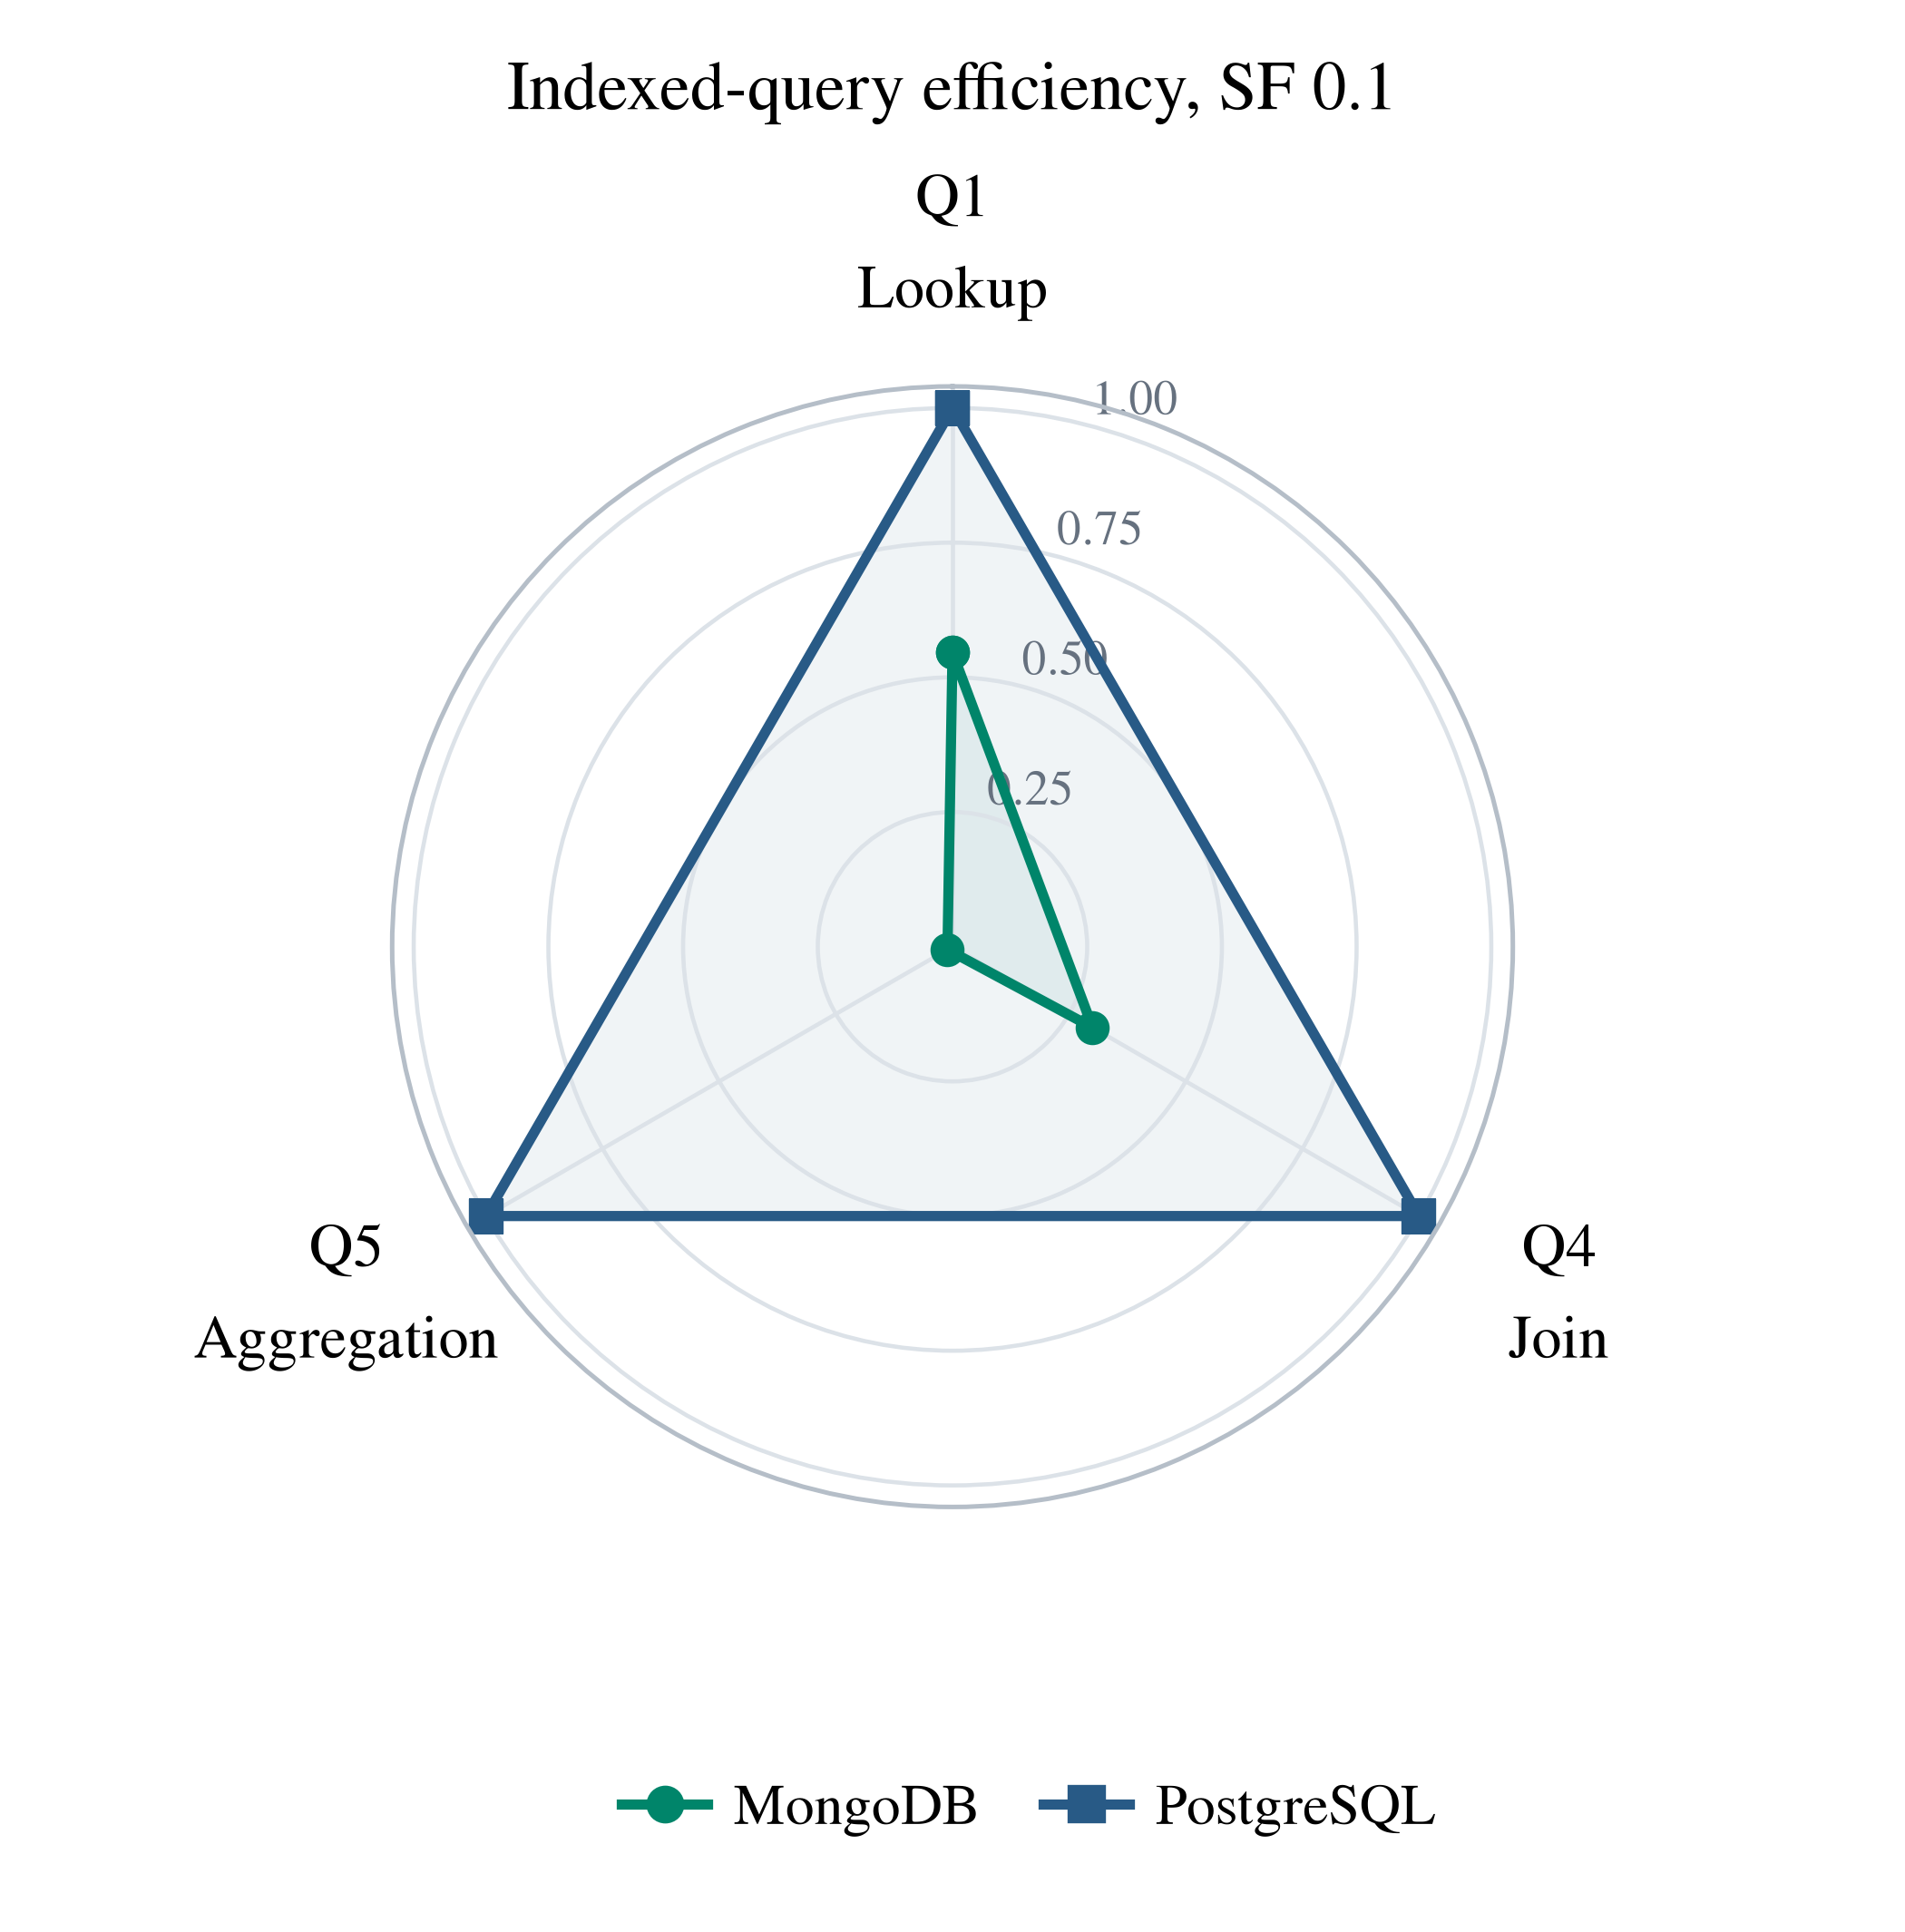
\includegraphics[width=\linewidth]{fig14_engine_capability_radar.png}
  \caption{Indexed-query latency efficiency at SF~0.1. A score of 1 identifies the faster median for an output-validated comparison. Resource efficiency is unmeasured.}
  \label{fig:radar}
\end{figure}

\begin{itemize}
  \item \textbf{Choose MongoDB for:} document-oriented access and schema flexibility when these match application requirements. The measured local MongoDB timings in Table~\ref{tab:master} determine its performance in the tested deployment.
  \item \textbf{Choose PostgreSQL for:} relational constraints and queries combining entities when these match application requirements. Its measured latency and storage are reported in the tables. The experiment does not quantify large-scale financial analytics or comparable engine-memory requirements.
\end{itemize}

% =====================================================================
\section*{Conclusion}
% =====================================================================

The study attempted the planned comparison across three scale factors (0.1, 0.5, and 1.0), three core workloads ($Q1$, $Q4$, and $Q5$), and two optional-index configurations. PostgreSQL had the lower observed median in 10 of the 10 complete core-query comparisons, and MongoDB in 0. Completed-comparison speedups ranged from $1.83\times$ to $232.46\times$. Both database servers ran on the same Windows host over loopback connections. The results characterize the recorded single-node settings, derived datasets, and warm-cache workloads. The evidence replaces formula-generated estimates with measured medians, recorded timeouts, and explicit unavailable values. Conclusions about H1--H5 require the corresponding volume, query, index, write, and storage measurements. A blanket confirmation of all hypotheses is not warranted by between-engine latency tests alone.

% =====================================================================
\section*{Limitations}
% =====================================================================

\textbf{Internal:} Repeated warm-cache runs, operating-system activity, other host activity, and fixed engine settings can affect timings~\cite{raasveldt2018fair}. \textbf{External:} The experiment targets SF~0.1--1.0 and a single local MongoDB deployment. Conditions that cannot finish loading or executing are identified in the evidence. \textbf{Construct:} Client latency includes driver, serialization, result transfer, and loopback network costs. PostgreSQL NUMERIC and MongoDB double arithmetic differ. Aggregate process RSS may double-count shared pages, and CPU accounting is coarse for short queries. Baseline primary-key access paths differ between engines, and configured cache budgets are unequal. \textbf{Scope:} $Q2$ and $Q3$ and detailed CRUD measurements are supplied in the evidence and figures. The core latency table retains $Q1$, $Q4$, and $Q5$. Local query identifiers differ from the standard TPC-H query numbering.

% =====================================================================
\section*{Future Work}
% =====================================================================

\begin{itemize}
  \item Extend the analysis of $Q2$ and $Q3$ to a controlled range of nonempty predicate selectivities.
  \item Compare deeply nested or denormalized MongoDB schemas with the corresponding set of normalized PostgreSQL tables.
  \item Stress-test both engines on multi-terabyte datasets in clusters with 10\,Gbps network links.
  \item Measure throughput at high concurrency using OLTP-Bench~\cite{difallah2013oltpbench}.
  \item Quantify the cost of distributed consensus under simultaneous reads and writes.
\end{itemize}

% =====================================================================
% REFERENCES
% =====================================================================
\begin{thebibliography}{30}

\bibitem{stonebraker2005c}
M.~Stonebraker and U.~\c{C}etintemel, ```One Size Fits All': An Idea Whose Time Has Come
and Gone,'' in \emph{Proc.\ Int.\ Conf.\ Data Engineering (ICDE)}, 2005, pp.~2--11.

\bibitem{pavlo2016relational}
A.~Pavlo and M.~Aslett, ``What's Really New with NewSQL?,'' \emph{ACM SIGMOD Record},
vol.~45, no.~2, pp.~45--55, 2016.

\bibitem{codd1970relational}
E.~F.~Codd, ``A Relational Model of Data for Large Shared Data Banks,''
\emph{Communications of the ACM}, vol.~13, no.~6, pp.~377--387, 1970.

\bibitem{postgresql_docs}
The PostgreSQL Global Development Group, ``PostgreSQL 18 Documentation,'' accessed Nov.\ 13, 2026. [Online].
Available: \url{https://www.postgresql.org/docs/18/}

\bibitem{postgresql_explain}
The PostgreSQL Global Development Group, ``PostgreSQL 18 EXPLAIN Documentation,'' accessed Nov.\ 13, 2026.
[Online]. Available: \url{https://www.postgresql.org/docs/18/sql-explain.html}

\bibitem{mongodb_docs}
MongoDB, Inc., ``MongoDB 8.0 Manual,'' accessed Nov.\ 13, 2026. [Online]. Available:
\url{https://www.mongodb.com/docs/v8.0/}

\bibitem{mongodb_aggregation}
MongoDB, Inc., ``Aggregation Pipeline --- MongoDB 8.0 Manual,'' accessed Nov.\ 13, 2026. [Online]. Available:
\url{https://www.mongodb.com/docs/v8.0/core/aggregation-pipeline/}

\bibitem{mongodb_explain}
MongoDB, Inc., ``Explain Results --- MongoDB 8.0 Manual,'' accessed Nov.\ 13, 2026. [Online]. Available:
\url{https://www.mongodb.com/docs/v8.0/reference/explain-results/}

\bibitem{cattell2011scalable}
R.~Cattell, ``Scalable SQL and NoSQL Data Stores,'' \emph{ACM SIGMOD Record}, vol.~39,
no.~4, pp.~12--27, 2011.

\bibitem{stonebraker2007end}
M.~Stonebraker \emph{et al.}, ``The End of an Architectural Era (It's Time for a Complete
Rewrite),'' in \emph{Proc.\ 33rd Int.\ Conf.\ Very Large Data Bases (VLDB)}, 2007, pp.~1150--1160.

\bibitem{sadalage2012nosql}
P.~J.~Sadalage and M.~Fowler, \emph{NoSQL Distilled: A Brief Guide to the Emerging World
of Polyglot Persistence}. Addison-Wesley, 2012.

\bibitem{leavitt2010nosql}
N.~Leavitt, ``Will NoSQL Databases Live Up to Their Promise?,'' \emph{IEEE Computer},
vol.~43, no.~2, pp.~12--14, 2010.

\bibitem{mohamed2014relational}
M.~A.~Mohamed, O.~G.~Altrafi, and M.~O.~Ismail, ``Relational vs.\ NoSQL Databases:
A Survey,'' \emph{Int.\ J.\ Computer and Information Technology}, vol.~3, no.~3,
pp.~598--601, 2014.

\bibitem{han2011survey}
J.~Han \emph{et al.}, ``Survey on NoSQL Database,'' in \emph{Proc.\ 6th Int.\ Conf.\
Pervasive Computing and Applications (ICPCA)}, 2011, pp.~363--366.

\bibitem{gessert2017nosql}
F.~Gessert, W.~Wingerath, S.~Friedrich, and N.~Ritter, ``NoSQL Database Systems:
A Survey and Decision Guidance,'' \emph{Computer Science --- Research and Development},
vol.~32, no.~3--4, pp.~353--365, 2017.

\bibitem{gyorodi2015comparative}
C.~Gy\H{o}r\"{o}di \emph{et al.}, ``A Comparative Study: MongoDB vs.\ MySQL,'' in
\emph{Proc.\ 13th Int.\ Conf.\ Engineering of Modern Electric Systems (EMES)}, 2015,
pp.~1--6.

\bibitem{parker2013comparing}
Z.~Parker, S.~Poe, and S.~V.~Vrbsky, ``Comparing NoSQL MongoDB to an SQL DB,'' in
\emph{Proc.\ 51st ACM Southeast Conf.\ (ACMSE)}, 2013, pp.~1--6.

\bibitem{jung2015mongodb}
M.-G.~Jung \emph{et al.}, ``A Study on Data Input and Output Performance Comparison of
MongoDB and PostgreSQL in the Big Data Environment,'' in \emph{Proc.\ 8th Int.\ Conf.\
Database Theory and Application (DTA)}, 2015, pp.~14--17.

\bibitem{boicea2012mongodb}
A.~Boicea, F.~Radulescu, and L.~I.~Agapin, ``MongoDB vs Oracle --- Database
Comparison,'' in \emph{Proc.\ 3rd Int.\ Conf.\ Emerging Intelligent Data and Web
Technologies (EIDWT)}, 2012, pp.~330--335.

\bibitem{li2013performance}
Y.~Li and S.~Manoharan, ``A Performance Comparison of SQL and NoSQL Databases,'' in
\emph{IEEE PACRIM}, 2013, pp.~15--19.

\bibitem{abramova2013nosql}
V.~Abramova and J.~Bernardino, ``NoSQL Databases: MongoDB vs Cassandra,'' in
\emph{Proc.\ C3S2E}, 2013, pp.~14--22.

\bibitem{cooper2010ycsb}
B.~F.~Cooper \emph{et al.}, ``Benchmarking Cloud Serving Systems with YCSB,'' in
\emph{Proc.\ 1st ACM Symp.\ Cloud Computing (SoCC)}, 2010, pp.~143--154.

\bibitem{difallah2013oltpbench}
D.~E.~Difallah, A.~Pavlo, C.~Curino, and P.~Cudre-Mauroux, ``OLTP-Bench: An Extensible
Testbed for Benchmarking Relational Databases,'' \emph{Proc.\ VLDB Endowment}, vol.~7,
no.~4, pp.~277--288, 2013.

\bibitem{raasveldt2018fair}
M.~Raasveldt \emph{et al.}, ``Fair Benchmarking Considered Difficult: Common Pitfalls in
Database Performance Testing,'' in \emph{Proc.\ DBTest Workshop}, 2018, pp.~1--6.

\bibitem{truica2015performance}
C.-O.~Truic\u{a} \emph{et al.}, ``Performance Evaluation for CRUD Operations in
Asynchronously Replicated Document Oriented Database,'' in \emph{Proc.\ 20th CSCS},
2015, pp.~191--196.

\bibitem{chaudhuri1998overview}
S.~Chaudhuri, ``An Overview of Query Optimization in Relational Systems,'' in
\emph{Proc.\ ACM PODS}, 1998, pp.~34--43.

\bibitem{graefe2011modern}
G.~Graefe, ``Modern B-Tree Techniques,'' \emph{Foundations and Trends in Databases},
vol.~3, no.~4, pp.~203--402, 2011.

\bibitem{tpch_spec}
Transaction Processing Performance Council, ``TPC Benchmark~H (Decision Support)
Standard Specification, Revision~3.0.1,'' 2022. [Online]. Available:
\url{https://www.tpc.org/tpch/}

\bibitem{poess2000tpch}
M.~Poess and C.~Floyd, ``New TPC Benchmarks for Decision Support and Web Commerce,''
\emph{ACM SIGMOD Record}, vol.~29, no.~4, pp.~64--71, 2000.

\bibitem{mann1947test}
H.~B.~Mann and D.~R.~Whitney, ``On a Test of Whether One of Two Random Variables is
Stochastically Larger than the Other,'' \emph{The Annals of Mathematical Statistics},
vol.~18, no.~1, pp.~50--60, 1947.

\end{thebibliography}

% Closing ornament
\begin{center}
\vspace{14pt}
$\bigstar\;\bigstar\;\bigstar$
\end{center}

% Author verification notes accompany this source.
\end{document}
